\section{Casi d'uso}
\subsection{Introduzione}
Nella seguente sezione vengono esposti i \glspl{usecase}\textsubscript{G} individuati. Ogni \gls{usecase}\textsubscript{G} viene descritto attraverso diagrammi dei \glspl{usecase}\textsubscript{G} e rappresenta uno \gls{scenario}\textsubscript{G} di utilizzo da parte degli \glspl{attore}\textsubscript{G} che si interfacciano con esso.
\subsection{Attori primari}
\begin{figure}[H]
	\centering
	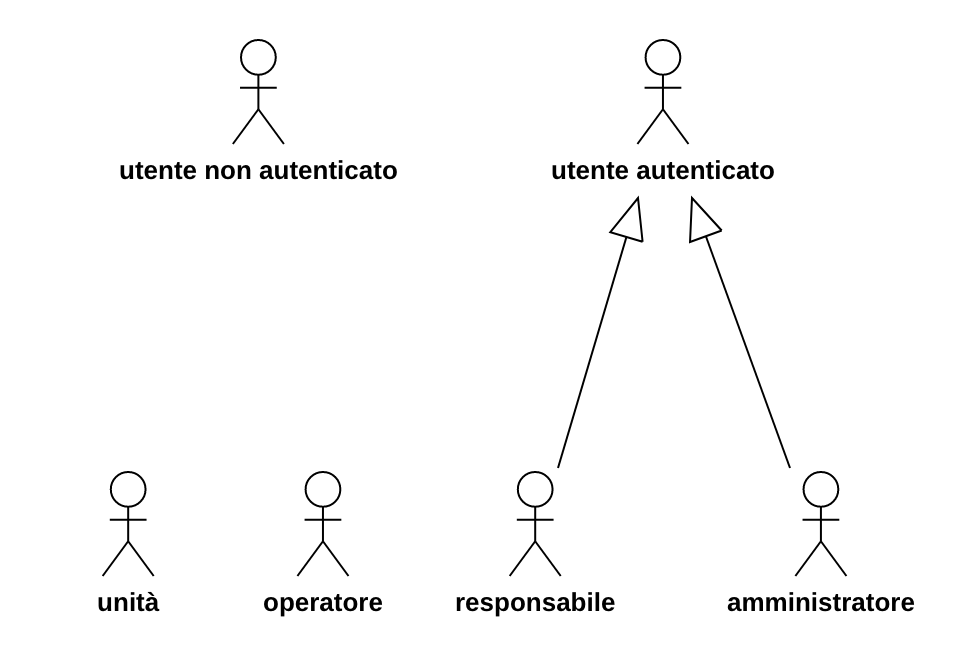
\includegraphics[scale=0.52]{res/images/gerarchia.png}
	\caption{Attori primari}
\end{figure}
\begin{itemize}
	\item{\textbf{Utente non autenticato:}\\
	Si riferisce ad un utente generico che non ha ancora effettuato l'accesso all'applicativo.}
	\item{\textbf{Utente autenticato:}\\
	Si riferisce ad un utente generico che ha effettuato l'accesso all'applicativo tramite il codice identificativo generato al momento dell'iscrizione;}
	\item{\textbf{Operatore:}\\
	Si riferisce all'utente autenticato che intraprende le azioni dirette con la macchina. Può quindi scegliere se guidare l'unità oppure servissi del pilota automatico per evadere i \glspl{task}\textsubscript{G}.}
	\item{\textbf{Responsabile:}\\
	 \'E la figura in capo della logistica del magazzino: inserisce i \glspl{task}\textsubscript{G} che devono essere svolti dagli operatori.}
	\item{\textbf{Amministratore:}\\
 Ha in capo la gestione operativa: inserisce, modifica ed elimina gli account del personale per l'accesso al sistema, censisce i muletti nel database, crea e modifica la\gls{planimetria}\textsubscript{G} e la percorribilità della mappa del magazzino.}
\end{itemize}

\subsection{UC1 - Login}
\begin{figure}[H]
	\centering
	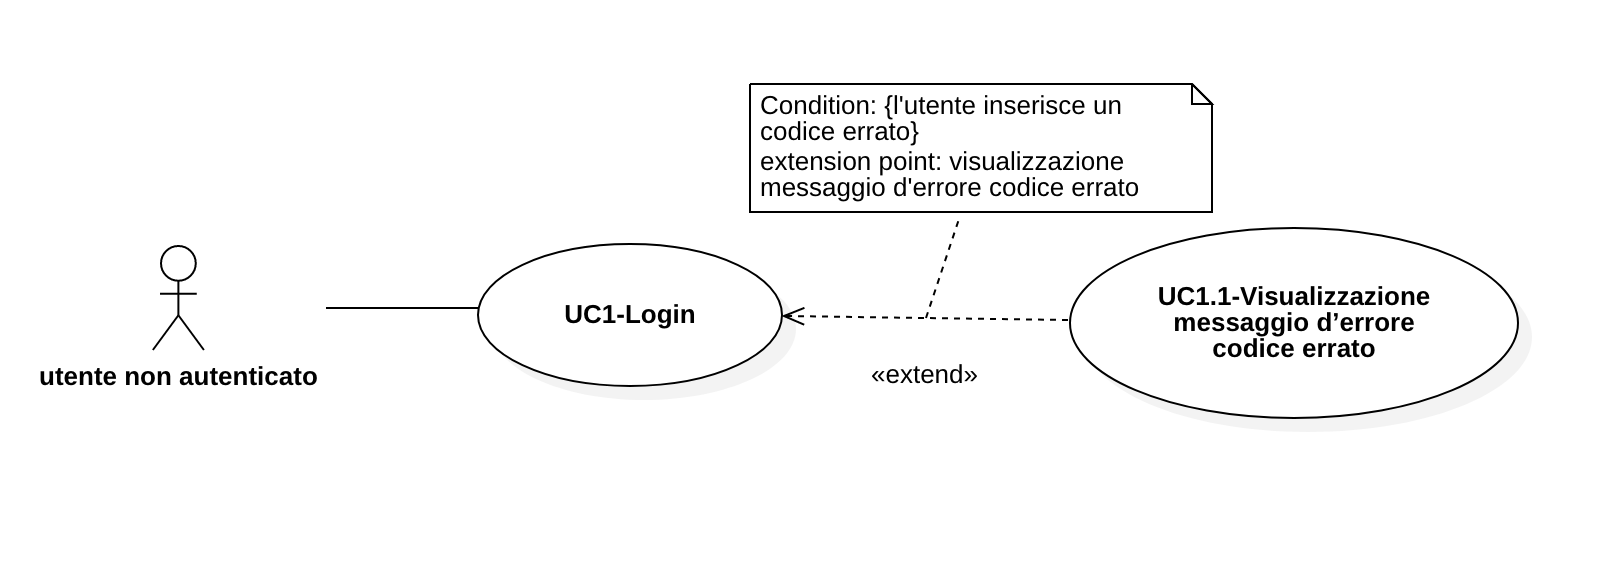
\includegraphics[scale=0.52]{res/images/uc1.png}
	\caption{UC1 - Login}
\end{figure}


\begin{itemize}
	\item 	\textbf{Attori primari:} utente non autenticato;
	\item 	\textbf{Precondizioni:} l'utente non è autenticato nell'applicativo;
	\item 	\textbf{Postcondizioni:}	l'utente si è autenticato con successo come operatore, responsabile o amministratore. Il sistema rende disponibili diverse pagine e funzionalità a seconda della tipologia di utente;
	\item 	\textbf{Scenario principale:} l'utente richiede il login inserendo nell'apposito \gls{form}\textsubscript{G} il proprio codice personale identificativo;
	\item 	\textbf{Descrizione:} l'utente tenta di autenticarsi attraverso il suo codice personale identificativo;
	\item 	\textbf{Estensioni:} 
		\begin{itemize}
			\item UC1.1: il codice non è stato inserito correttamente dal sistema e quindi viene visualizzato un messaggio d'errore.
		\end{itemize}
\end{itemize}
\subsubsection{UC1.1 - Visualizzazione messaggio d'errore codice errato}

\begin{itemize}
	\item 	\textbf{Attori primari:} utente non autenticato;
	\item 	\textbf{Precondizioni:} l'utente ha inserito il suo codice personale identificativo;
	\item 	\textbf{Postcondizioni:} viene visualizzato un messaggio d'errore che informa l'utente che il codice identificativo è errato e di riprovare;
	\item 	\textbf{Scenario principale:} l'utente tenta di autenticarsi inserendo un codice non presente nel sistema o errato;
	\item 	\textbf{Descrizione:} l'utente visualizza un messaggio d'errore dopo aver inserito un codice errato o non presente nel sistema; quindi gli viene chiesto di riprovare o di recarsi dall'amministratore.
	
\end{itemize}

\subsection{UC2 - Registrazione nuovo utente}

\begin{figure}[H]
	\centering
	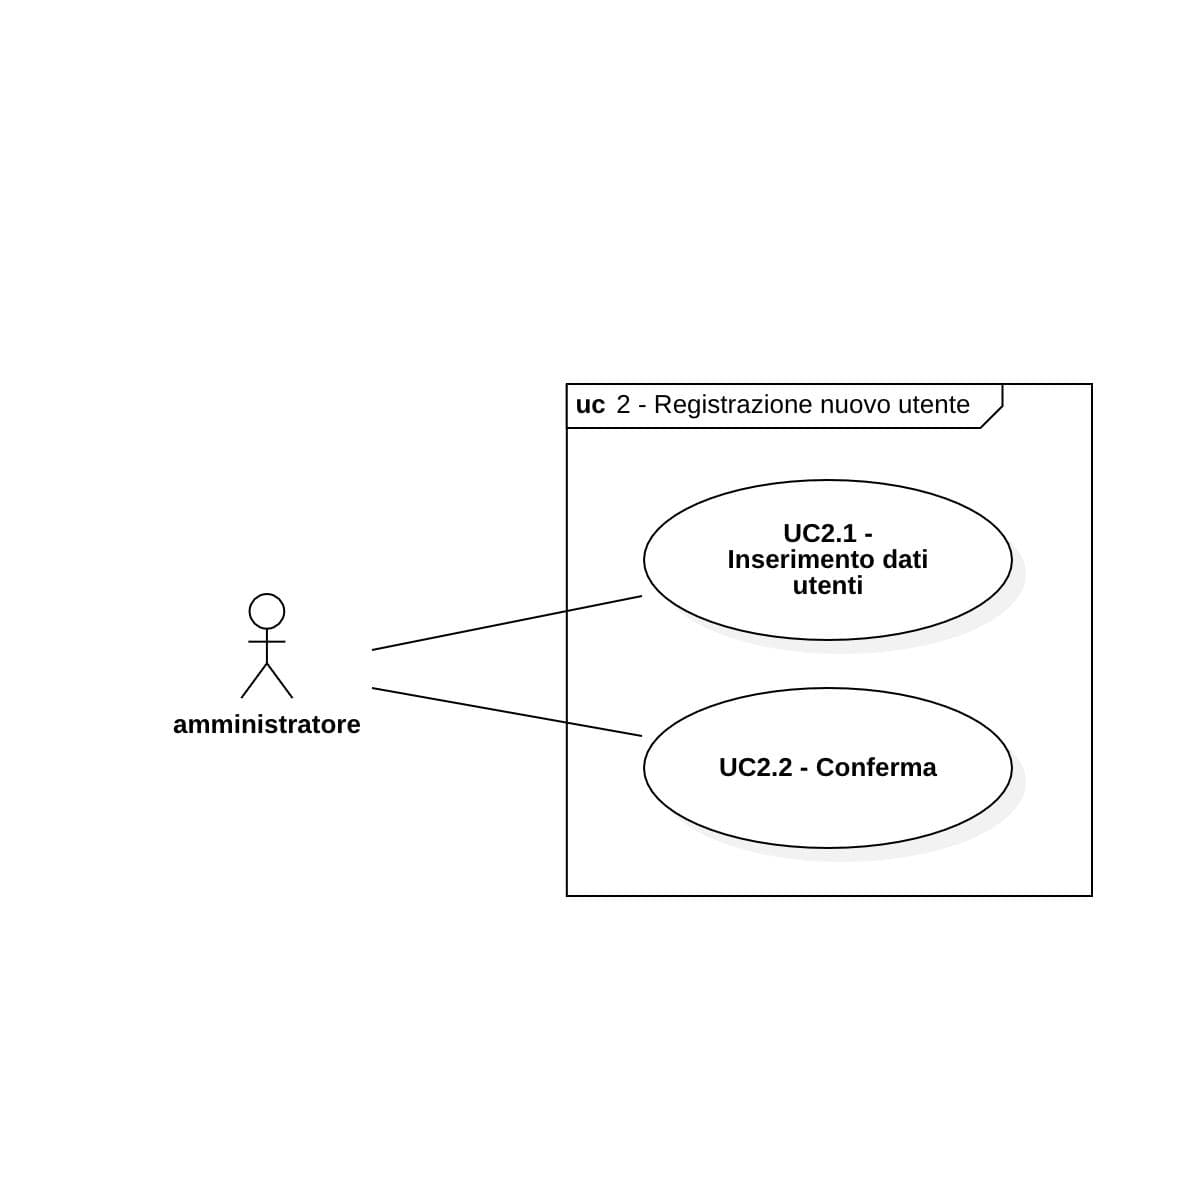
\includegraphics[scale=0.52]{res/images/uc2.png}
	\caption{UC2 - Registrazione nuovo utente}
\end{figure}
\begin{itemize}
	\item 	\textbf{Attori primari:} amministratore;
	\item 	\textbf{Precondizioni:}	l'amministratore intende registrare nel sistema un nuovo lavoratore assunto nell'azienda non ancora registrato nell'applicativo.
	\item 	\textbf{Postcondizioni:} l'utente è registrato nel sistema correttamente come responsabile o operatore;
	\item 	\textbf{Scenario principale:} l'amministratore inserisce i dati personali del lavoratore che vuole registrare nell'applicativo specificandone il ruolo che deve ricoprire all'interno del magazzino (responsabile o operatore);
	\item 	\textbf{Descrizione:} per effettuare l'aggiunta di un nuovo utente, l'amministratore deve compilare i dati dell'account che non devono essere presente all'interno del sistema. Il nuovo utente può essere un responsabile o un operatore.

\end{itemize}

\subsubsection{UC2.1 - Inserimento dati utente}

\begin{figure}[H]
	\centering
	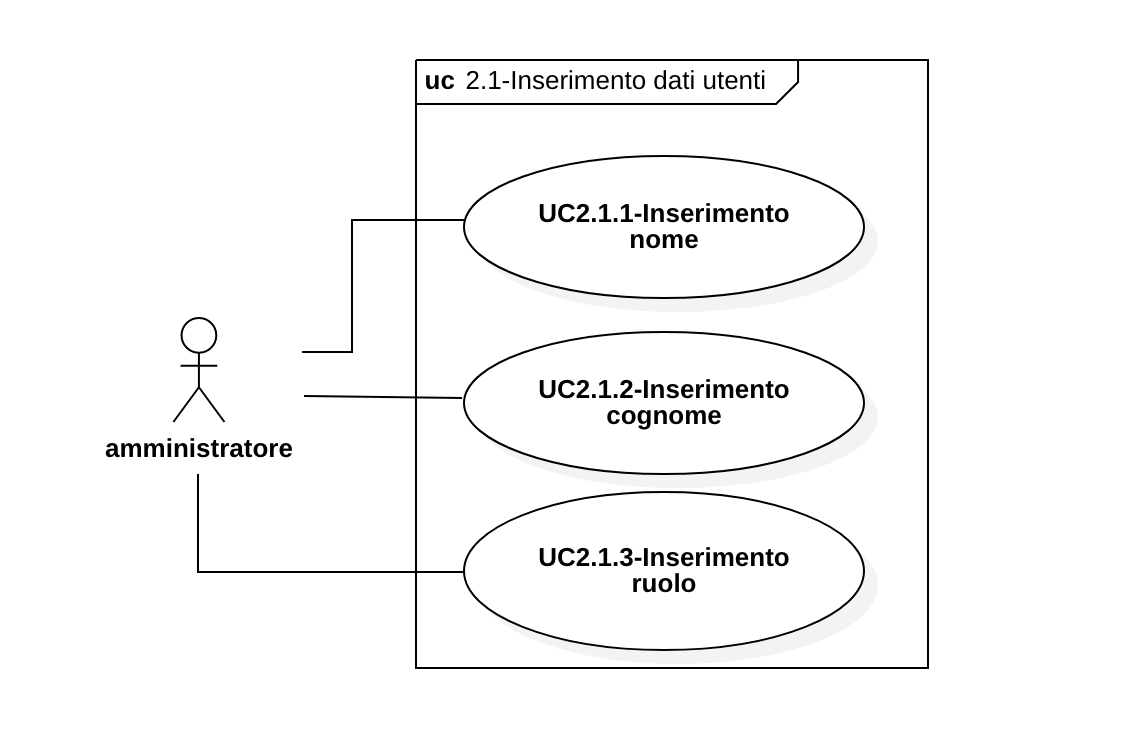
\includegraphics[scale=0.52]{res/images/uc2-1.png}
	\caption{UC2.1 - Inserimento dati utente}
\end{figure}

\begin{itemize}
	\item 	\textbf{Attori primari:} amministratore;
	\item 	\textbf{Precondizioni:}	l'amministratore sta eseguendo la registrazione del lavoratore nel sistema;
	\item 	\textbf{Postcondizioni:} l'amministratore ha inserito tutti i campi del \gls{form}\textsubscript{G} di registrazione richiesti;
	\item 	\textbf{Scenario principale:} l'amministratore compila tutti i campi del \gls{form}\textsubscript{G} richiesti per la registrazione, ovvero:
	\begin{itemize}
		\item inserisce il nome del lavoratore (UC2.1.1);
		\item inserisce il cognome del lavoratore (UC2.1.2);
		\item inserisce il ruolo del lavoratore, ovverosia operatore o responsabile (UC2.1.3);
	\end{itemize}
	\item 	\textbf{Descrizione:} per effettuare la registrazione, l'amministratore deve fornire i seguenti dati dell'utente:
	\begin{itemize}
		\item nome;
		\item cognome
		\item ruolo (responsabile, operatore).
	\end{itemize}

\end{itemize}

\paragraph{UC2.1.1 - Inserimento nome}
\begin{itemize}
	\item 	\textbf{Attori primari:} amministratore;
	\item 	\textbf{Precondizioni:} il sistema ha reso disponibile il campo del \gls{form}\textsubscript{G} per inserire il nome del lavoratore;
	\item 	\textbf{Postcondizioni:} l'amministratore ha compilato il campo con il nome;
	\item 	\textbf{Scenario principale:} l'amministratore compila il campo del \gls{form}\textsubscript{G} relativo al nome del lavoratore;
	\item 	\textbf{Descrizione:} per effettuare l'aggiunta di un nuovo utente, l'amministratore deve inserire il nome del lavoratore che si intende registrare.

\end{itemize}

\paragraph{UC2.1.2 - Inserimento cognome}

\begin{itemize}
	\item 	\textbf{Attori primari:} amministratore;
	\item 	\textbf{Precondizioni:} il sistema ha reso disponibile il campo del \gls{form}\textsubscript{G} per inserire il cognome del lavoratore;
	\item 	\textbf{Postcondizioni:} l'amministratore ha compilato il campo con il cognome;
	\item 	\textbf{Scenario principale:} l'amministratore compila il campo del \gls{form}\textsubscript{G} relativo al cognome del lavoratore;
	\item 	\textbf{Descrizione:} per effettuare l'aggiunta di un nuovo utente, l'amministratore deve inserire il cognome del lavoratore che si intende registrare.
	
\end{itemize}

\paragraph{UC2.1.3 - Inserimento ruolo}

\begin{itemize}
	\item 	\textbf{Attori primari:} amministratore;
	\item 	\textbf{Precondizioni:} il sistema ha reso disponibile il campo del \gls{form}\textsubscript{G} per inserire il ruolo del lavoratore;
	\item 	\textbf{Postcondizioni:} l'amministratore ha compilato il campo con il ruolo;
	\item 	\textbf{Scenario principale:} l'amministratore sceglie tramite una \gls{combobox}\textsubscript{G} il ruolo che dovrà intraprendere il nuovo lavoratore, ovverosia responsabile o operatore;
	\item 	\textbf{Descrizione:} per effettuare l'aggiunta di un nuovo utente, l'amministratore deve inserire il ruolo del lavoratore che si intende registrare. Può scegliere tra responsabile e operatore.
	
\end{itemize}


\subsubsection{UC2.2 - Conferma}

\begin{itemize}
	\item 	\textbf{Attori primari:} amministratore;
	\item 	\textbf{Precondizioni:} l'amministratore ha compilato il \gls{form}\textsubscript{G} per l'inserimento dei dati del nuovo utente e rende disponibile un pulsante per la conferma;
	\item 	\textbf{Postcondizioni:} viene visualizzato a video un messaggio con la conferma della ricezione dei dati e il codice identificativo;
	\item 	\textbf{Scenario principale:} l'amministratore preme il pulsante di conferma dopo aver completato tutti i campi del \gls{form}\textsubscript{G};
	\item 	\textbf{Descrizione:} l'amministratore preme il pulsante per la conferma dell'inserimento dei dati. A schermo viene visualizzato un messaggio con l'avvenuta registrazione e il codice identificativo relativo all'account registrato.

\end{itemize}

\subsubsection{UC2.3 - Visualizzazione messaggio d'errore account già presente}

\begin{itemize}
	\item 	\textbf{Attori primari:} amministratore;
	\item 	\textbf{Precondizioni:} i dati del lavoratore sono già presenti nel sistema;
	\item 	\textbf{Postcondizioni:} viene visualizzato a video un messaggio d'errore per informare l'amministratore che il lavoratore è già presente nel sistema;
	\item 	\textbf{Scenario principale:} l'amministratore tenta di registrare nell'applicativo un lavoratore già registrato;
	\item 	\textbf{Descrizione:} l'amministratore visualizza un messaggio d'errore dovuto al fatto di aver inserito i dati di un utente già presente nel sistema.
\end{itemize}

\subsection{UC3 - Gestione account già presenti}
\begin{figure}[H]
	\centering
	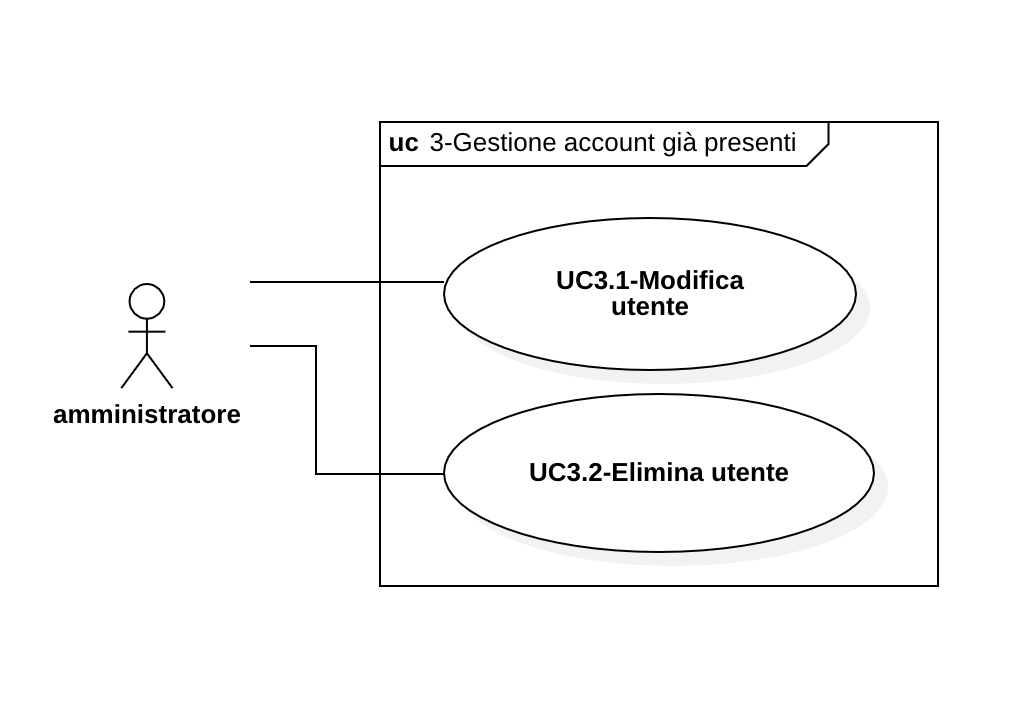
\includegraphics[scale=0.52]{res/images/uc3.png}
	\caption{UC3 - Gestione account già presenti}
\end{figure}

\begin{itemize}
	\item 	\textbf{Attori primari:} amministratore;
	\item 	\textbf{Precondizioni:} l'amministratore intende effettuare un cambiamento degli account già presenti nel sistema;
	\item 	\textbf{Postcondizioni:} vi è un cambiamento degli account registrati;
	\item 	\textbf{Scenario principale:} vengono visualizzate le operazioni che l'amministratore può effettuare per gestire gli account già presenti:
	\begin{itemize}
		\item modificare i dati di un utente (UC3.1);
		\item eliminare l'account di un utente (UC3.2).
	\end{itemize}
	Viene poi mostrato un \gls{form}\textsubscript{G} di ricerca per inserire il codice identificativo dell'utente interessato;
	\item 	\textbf{Descrizione:} l'amministratore ha il compito di gestire gli account presenti nel sistema e aggiornarli in base all'organico del magazzino.
\end{itemize}

\subsubsection{UC3.1 - Modifica utente}

\begin{figure}[H]
	\centering
	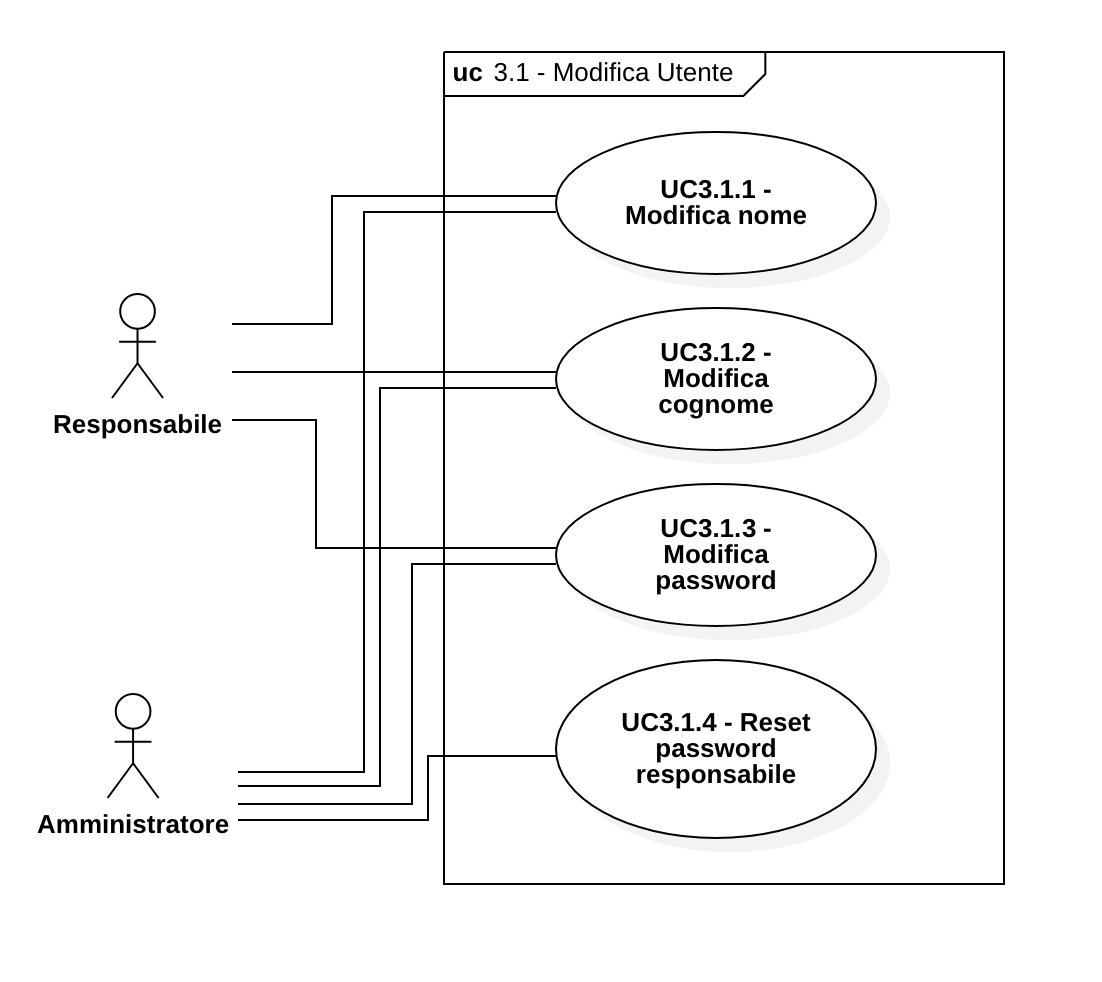
\includegraphics[scale=0.52]{res/images/uc3-1.png}
	\caption{UC3.1 - Modifica utente}
\end{figure}
\begin{itemize}
	\item 	\textbf{Attori primari:} amministratore;
	\item 	\textbf{Precondizioni:} l'amministratore intende modificare il profilo dell'utente selezionato già registrato all'interno dell'applicativo;
	\item 	\textbf{Postcondizioni:} l'amministratore ha cambiato alcuni campi dell'account di un utente;
	\item 	\textbf{Scenario principale:} l'amministratore modifica un campo del profilo dell'utente;
	\item 	\textbf{Descrizione:} per modificare un campo dell'account di un lavoratore, l'amministratore deve modificare quello corrente con quello corretto.

\end{itemize}

\paragraph{UC3.1.1 - Modifica nome}

\begin{itemize}
	\item 	\textbf{Attori primari:} amministratore;
	\item 	\textbf{Precondizioni:} il sistema ha reso disponibile il campo del \gls{form}\textsubscript{G} per modificare il nome del lavoratore;
	\item 	\textbf{Postcondizioni:}  l'amministratore ha compilato il campo con il nome aggiornato;
	\item 	\textbf{Scenario principale:} l'amministratore compila il campo del \gls{form}\textsubscript{G} relativo al nome del lavoratore con il nome aggiornato;
	\item 	\textbf{Descrizione:} per effettuare la modifica del campo relativo al nome del lavoratore, l'amministratore aggiorna il \gls{form}\textsubscript{G}.
\end{itemize}

\paragraph{UC3.1.2 - Modifica cognome}

\begin{itemize}
	\item 	\textbf{Attori primari:} amministratore;
	\item 	\textbf{Precondizioni:} il sistema ha reso disponibile il campo del \gls{form}\textsubscript{G} per modificare il cognome del lavoratore;
	\item 	\textbf{Postcondizioni:} l'amministratore ha compilato il campo con il cognome aggiornato;
	\item 	\textbf{Scenario principale:} l'amministratore compila il campo del \gls{form}\textsubscript{G} relativo al cognome del lavoratore con il cognome aggiornato;
	\item 	\textbf{Descrizione:} per effettuare la modifica del campo relativo al cognome del lavoratore, l'amministratore aggiorna il \gls{form}\textsubscript{G}.

\end{itemize}
\paragraph{UC3.1.3 - Modifica ruolo}

\begin{itemize}
	\item 	\textbf{Attori primari:} amministratore;
	\item 	\textbf{Precondizioni:} il sistema ha reso disponibile il campo del \gls{form}\textsubscript{G} per modificare il ruolo del lavoratore;
	\item 	\textbf{Postcondizioni:} l'amministratore ha compilato il campo con il ruolo aggiornato (responsabile o operatore);
	\item 	\textbf{Scenario principale:} l'amministratore compila il campo del \gls{form}\textsubscript{G} relativo al ruolo del lavoratore con il ruolo aggiornato scegliendo tra responsabile o operatore;
	\item 	\textbf{Descrizione:} per effettuare la modifica del campo relativo al ruolo del lavoratore, l'amministratore aggiorna il \gls{form}\textsubscript{G}.

\end{itemize}

\subsubsection{UC3.2 - Elimina utente}

\begin{itemize}
	\item 	\textbf{Attori primari:} amministratore;
	\item 	\textbf{Precondizioni:} l'amministratore intende eliminare il profilo dell'utente selezionato;
	\item 	\textbf{Postcondizioni:} è stato eliminato dal sistema l'account dell'utente selezionato;
	\item 	\textbf{Scenario principale:} l'amministratore preme il pulsante apposito per l'eliminazione dell'account;
	\item 	\textbf{Descrizione:} può essere necessario eliminare l'account di un utente.
\end{itemize}

\subsection{UC4 - Gestione task}

\begin{figure}[H]
	\centering
	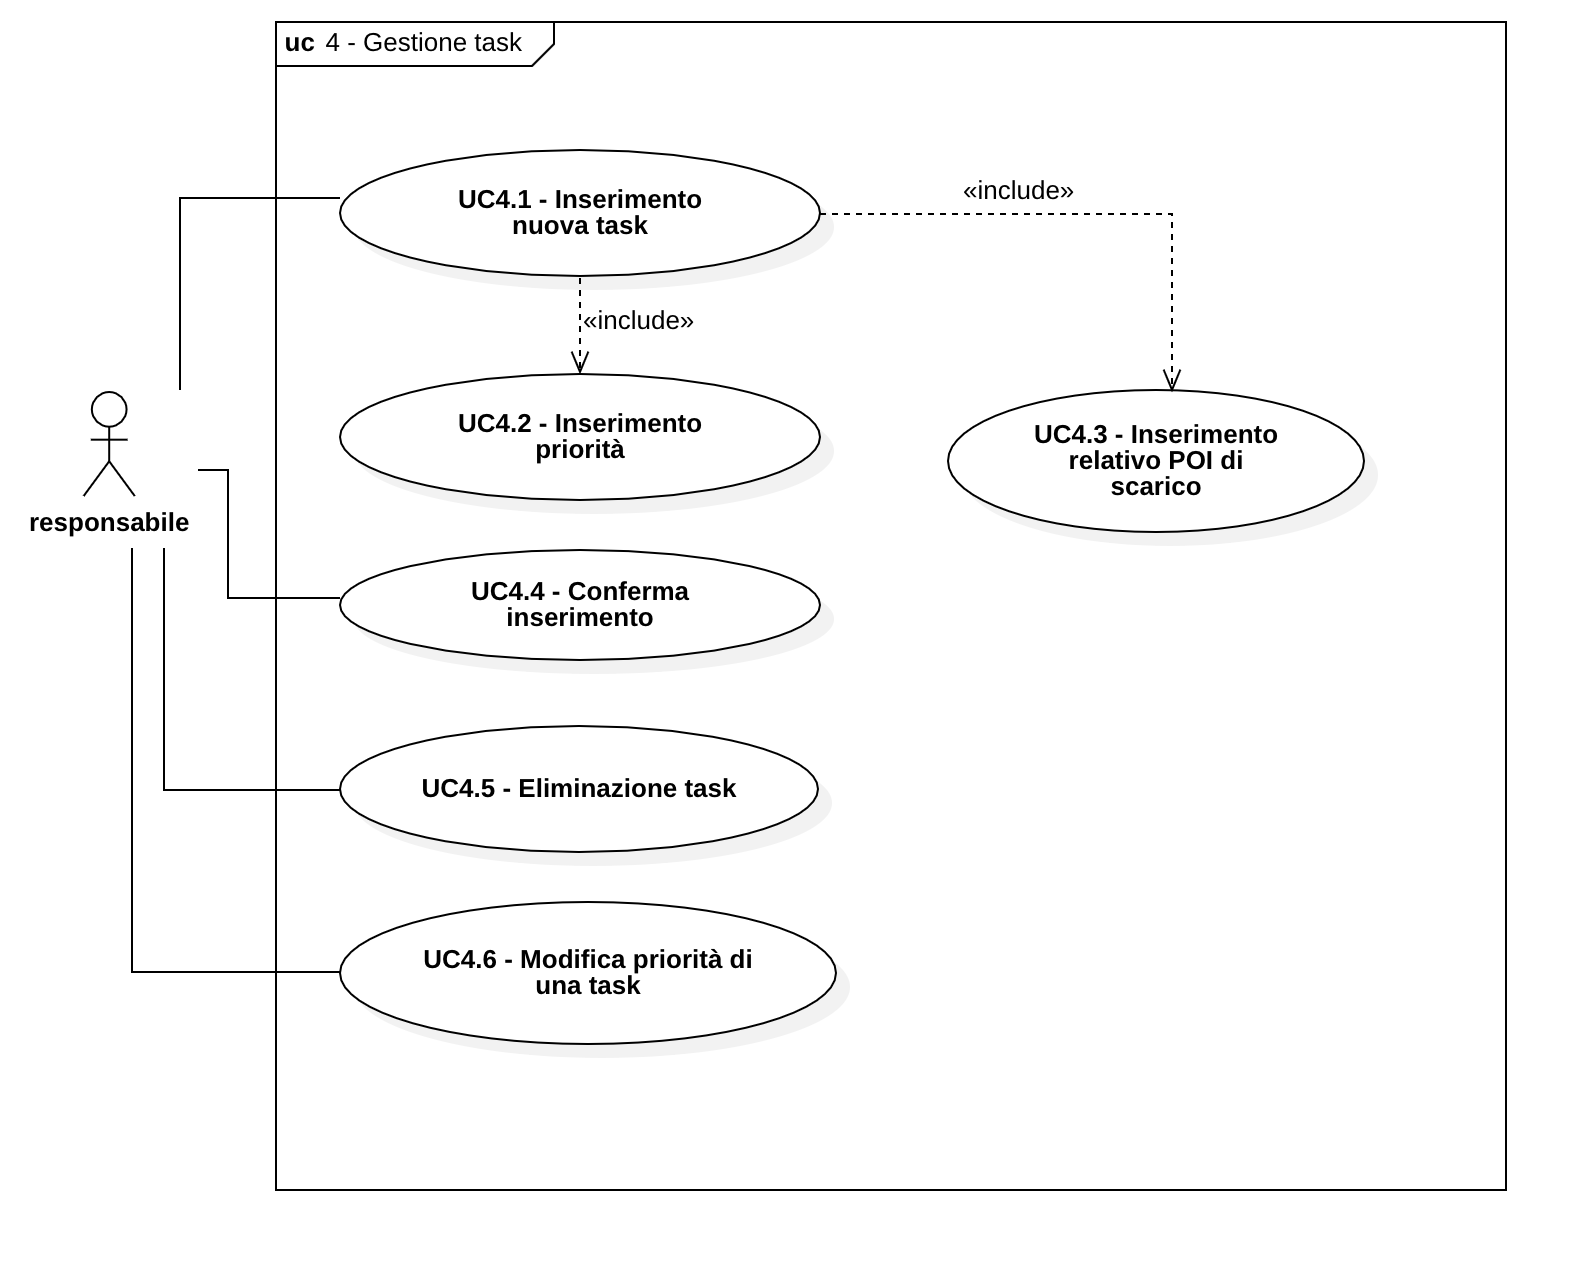
\includegraphics[scale=0.52]{res/images/uc4.png}
	\caption{UC4 - Gestione task}
\end{figure}

\begin{itemize}
	\item 	\textbf{Attori primari:} responsabile;
	\item 	\textbf{Precondizioni:} il responsabile è autenticato nel sistema e il sistema rende disponibile l'interfaccia per la gestione delle \gls{task}\textsubscript{G} che verranno assegnati alle unità;
	\item 	\textbf{Postcondizioni:} la lista delle \gls{task}\textsubscript{G} è stata aggiornata;
	\item 	\textbf{Scenario principale:} il responsabile effettua le operazioni necessarie per la gestione della lista delle \gls{task}\textsubscript{G} che verranno assegnate dal sistema alle unità, esse possono essere:
	\begin{itemize}
		\item l'inserimento di una nuova \gls{task}\textsubscript{G} (UC4.1) con la relativa priorità (UC4.2) e il \acrshort{POI}\textsubscript{A} a cui fa riferimento, in cui bisogna scaricare la merce (UC4.3);
		\item la conferma dell'inserimento della nuova \gls{task}\textsubscript{G} (UC4.4);
		\item l'eliminazione di una \gls{task}\textsubscript{G} dalla lista (UC4.5);
		\item la modifica della priorità di una \gls{task}\textsubscript{G} esistente (UC4.6);
	\end{itemize}
	\item 	\textbf{Descrizione:} lo scarico delle merci in un determinato punto di interesse viene chiamato \gls{task}\textsubscript{G}. Il responsabile deve inserire nel sistema quali \gls{task}\textsubscript{G} devono essere completate e con quale priorità. L'applicativo riceve le informazioni, le ordina e le affida alle unità in base alle esigenze. 

\end{itemize}

\subsubsection{UC4.1 - Inserimento nuova task}

\begin{itemize}
	\item 	\textbf{Attori primari:} responsabile;
	\item 	\textbf{Precondizioni:} è resa disponibile l'interfaccia per l'inserimento di una nuova \gls{task}\textsubscript{G};
	\item 	\textbf{Postcondizioni:} il responsabile ha aggiunto con successo la \gls{task}\textsubscript{G} alla lista. Il sistema assegnerà la nuova \gls{task}\textsubscript{G} a un muletto, il quale la visualizzerà nella propria lista di compiti (UC8);
	\item 	\textbf{Scenario principale:} il responsabile preme l'apposito pulsante per l'aggiunta di una nuova \gls{task}\textsubscript{G}; 
	\item 	\textbf{Descrizione:} il responsabile inserisce un nuovo compito da eseguire nella lista dei \gls{task}\textsubscript{G};
	\item 	\textbf{Inclusioni:}
	\begin{itemize}
		\item UC4.2 Inserimento priorità;
		\item UC4.3 Inserimento relativo \acrshort{POI}\textsubscript{A}.
	\end{itemize}
\end{itemize}

\subsubsection{UC4.2 - Inserimento priorità}

\begin{itemize}
	\item 	\textbf{Attori primari:} responsabile;
	\item 	\textbf{Precondizioni:} il responsabile sta inserendo una nuova \gls{task}\textsubscript{G};
	\item 	\textbf{Postcondizioni:} è stata compilata correttamente la priorità relativa alla \gls{task}\textsubscript{G} che si vuole inserire;
	\item 	\textbf{Scenario principale:} il responsabile le assegna una priorità (bassa, media, alta) tramite una \gls{combobox}\textsubscript{G};
	\item 	\textbf{Descrizione:} le \gls{task}\textsubscript{G} possono avere tre diversi gradi di priorità:
	\begin{itemize}
		\item bassa;
		\item media;
		\item alta.
	\end{itemize}
\end{itemize}

\subsubsection{UC4.3 - Inserimento relativo \acrshort{POI}\textsubscript{A} di scarico}

\begin{itemize}
	\item 	\textbf{Attori primari:} responsabile;
	\item 	\textbf{Precondizioni:} il responsabile sta inserendo una nuova \gls{task}\textsubscript{G};
	\item 	\textbf{Postcondizioni:} è stato assegnato correttamente il \acrshort{POI}\textsubscript{A} relativo alla nuova \gls{task}\textsubscript{G};
	\item 	\textbf{Scenario principale:}
	\begin{itemize}
		\item visualizza la mappa con tutti i \acrshort{POI}\textsubscript{A} (UC6) e la lista di tutti i \acrshort{POI}\textsubscript{A} di scarico (UC12);
		\item seleziona il \acrshort{POI}\textsubscript{A} in cui si vuole scaricare la merce;
		\item viene confermata la selezione.
	\end{itemize}
	\item 	\textbf{Descrizione:} la \gls{task}\textsubscript{G} rappresenta lo scarico merci in un determinato punto di interesse del magazzino, quindi ad ogni \gls{task}\textsubscript{G} deve essere affidato il relativo \acrshort{POI}\textsubscript{A}.
\end{itemize}
\subsubsection{UC4.4 - Conferma inserimento}

\begin{itemize}
	\item 	\textbf{Attori primari:} responsabile;
	\item 	\textbf{Precondizioni:} il responsabile ha creato la nuova \gls{task}\textsubscript{G} e il sistema rende disponibile il pulsante di conferma;
	\item 	\textbf{Postcondizioni:} il sistema ha ricevuto la nuova \gls{task}\textsubscript{G} e lo assegna a un'unità che lo dovrà soddisfare;
	\item 	\textbf{Scenario principale:} il responsabile conferma l'inserimento della nuova \gls{task}\textsubscript{G} tramite un apposito pulsante;
	\item 	\textbf{Descrizione:} il responsabile visualizza il pulsante di conferma per inserire la \gls{task}\textsubscript{G}.
\end{itemize}

\subsubsection{UC4.5 - Eliminazione task}

\begin{itemize}
	\item 	\textbf{Attori primari:} responsabile;
	\item 	\textbf{Precondizioni:} il responsabile sta visualizzando la lista di \gls{task}\textsubscript{G} (UC13);
	\item 	\textbf{Postcondizioni:} il responsabile ha eliminato una \gls{task}\textsubscript{G} dalla lista;
	\item 	\textbf{Scenario principale:} il responsabile seleziona dalla lista delle \gls{task}\textsubscript{G} quella che intende eliminare e procede alla cancellazione premendo l'apposito pulsante;
	\item 	\textbf{Descrizione:} il responsabile si accorge che non è più necessario lo svolgimento di un compito, quindi lo elimina dalla lista delle \gls{task}\textsubscript{G}.

\end{itemize}

\subsubsection{UC4.6 - Modifica priorità di una task}
\begin{itemize}
	\item 	\textbf{Attori primari:} responsabile;
	\item 	\textbf{Precondizioni:} il responsabile sta visualizzando la lista di task(UC13);
	\item 	\textbf{Postcondizioni:} la priorità della \gls{task}\textsubscript{G} selezionata è stata aggiornata;
	\item 	\textbf{Scenario principale:} il responsabile seleziona la \gls{task}\textsubscript{G} che intende modificare, viene aperto un menu a tendina nel quale è possibile cambiare la priorità;
	\item 	\textbf{Descrizione:} il responsabile si accorge che la priorità di una \gls{task}\textsubscript{G} è errata o necessita di un aggiornamento, quindi procede con la modifica.
\end{itemize}

\subsection{UC5 - Logout}

\begin{itemize}
	\item 	\textbf{Attori primari:} utente autenticato;
	\item 	\textbf{Precondizioni:} l'utente si trova in base e quindi può premere sul bottone che gli permette di fare il logout dall'applicativo;
	\item 	\textbf{Postcondizioni:} l'utente viene disconnesso dal sistema;
	\item 	\textbf{Scenario principale:} utente autenticato richiede il logout;
	\item 	\textbf{Descrizione:} l'utente vuole effettuare il logout dall'applicativo:
	\begin{itemize}
		\item se amministratore o responsabile, può effettuare il logout dall'applicativo in qualsiasi momento;
		\item se operatore, può effettuare il logout solo dopo aver evaso tutti \glspl{task}\textsubscript{G} assegnati e raggiunto la base.
	\end{itemize}
\end{itemize}


\subsection{UC6 - Visualizzazione mappa}

\begin{figure}[H]
	\centering
	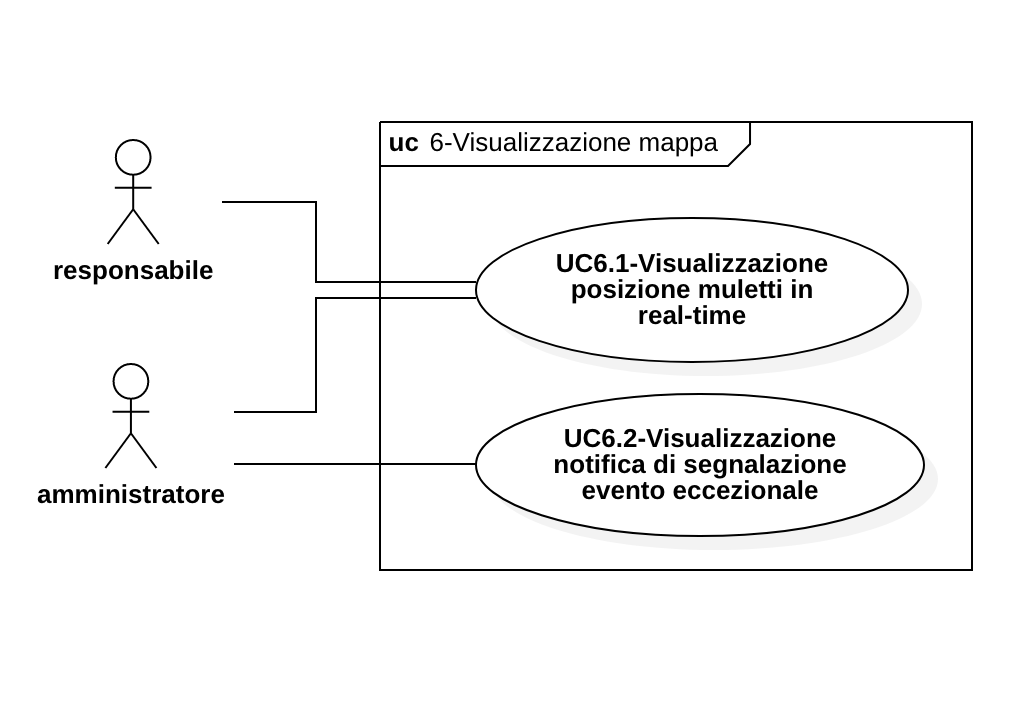
\includegraphics[scale=0.52]{res/images/uc6.png}
	\caption{UC6 - Visualizzazione mappa}
\end{figure}

\begin{itemize}
	\item 	\textbf{Attori primari:} amministratore, responsabile;
	\item 	\textbf{Precondizioni:} gli \glspl{attore}\textsubscript{G} sono autenticati nel sistema;
	\item 	\textbf{Postcondizioni:} gli \glspl{attore}\textsubscript{G} visualizzano la mappa del magazzino;
	\item 	\textbf{Scenario principale:} il responsabile e l'amministratore, una volta autenticati, visualizzano la mappa completa del magazzino;
	\item 	\textbf{Descrizione:} il responsabile e l'amministratore supervisionano il magazzino tramite una mappa che ne visualizza gli elementi strutturali. Gli elementi della mappa sono:
	\begin{itemize}
		\item \acrshort{POI}\textsubscript{A} di carico:  punto in cui i muletti prelevano il carico di merce da smistare nel magazzino. Ogni volta che completano la loro lista di \glspl{task}\textsubscript{G} (ma non è finito il loro turno di lavoro), devono tornare su questo punto per effettuare un nuovo carico e ricevere nuove \glspl{task}\textsubscript{G};
		\item \acrshort{POI}\textsubscript{A} di scarico: punti in cui i muletti devono scaricare la merce prelevata;
		\item \acrshort{POI}\textsubscript{A} di sosta o di base: punto in cui gli operatori partono con il proprio muletto a inizio turno e arrivano alla fine del turno.
		\item zona di \gls{percorrenza}\textsubscript{G}: strade in cui i muletti possono transitare, le cui caratteristiche sono:
		\begin{itemize}
			\item senso di marcia;
			\item numero massimo di unità che può transitare;
		\end{itemize}
		\item aree non transitabili: muri, scaffali, elementi e zone del magazzino che non prevedono il transito di un muletto.
	\end{itemize}

\end{itemize}


\subsubsection{UC6.1 - Visualizzazione posizione muletti in real-time}
\begin{itemize}
	\item 	\textbf{Attori primari:} amministratore, responsabile;
	\item 	\textbf{Precondizioni:} gli \glspl{attore}\textsubscript{G} sono autenticati nel sistema e visualizzano correttamente la mappa;
	\item 	\textbf{Postcondizioni:} gli \glspl{attore}\textsubscript{G} visualizzano gli spostamenti dei muletti in real-time nella mappa;
	\item 	\textbf{Scenario principale:} il responsabile e l'amministratore una volta autenticati, visualizzano la mappa completa del magazzino con i muletti in movimento;
	\item 	\textbf{Descrizione:} il responsabile e l'amministratore supervisionano il magazzino tramite una mappa che visualizza in real-time la posizione dei muletti al suo interno.
\end{itemize}

\subsubsection{UC6.2 - Visualizzazione notifica di segnalazione evento eccezionale}
\begin{itemize}
	\item 	\textbf{Attori primari:} amministratore;
	\item 	\textbf{Precondizioni:} è stato segnalato un evento eccezionale da un operatore;
	\item 	\textbf{Postcondizioni:} viene visualizzata una notifica che avverte l'amministratore dell'avvenimento un evento eccezionale;
	\item 	\textbf{Scenario principale:} il sistema visualizza una notifica di segnalazione dell'avvenimento di un evento eccezionale, evidenziando il punto in cui si è verificato;
	\item 	\textbf{Descrizione:} l'operatore mentre sta completando le proprie \gls{task}\textsubscript{G}, può segnalare l'avvenimento di un evento eccezionale all'interno del magazzino (UC11.3). Il sistema dovrà notificare l'amministratore di questo e indicargli la posizione in cui è stato riscontrato.
\end{itemize}

\subsection{UC7 - Gestione mappa}

\begin{figure}[H]
	\centering
	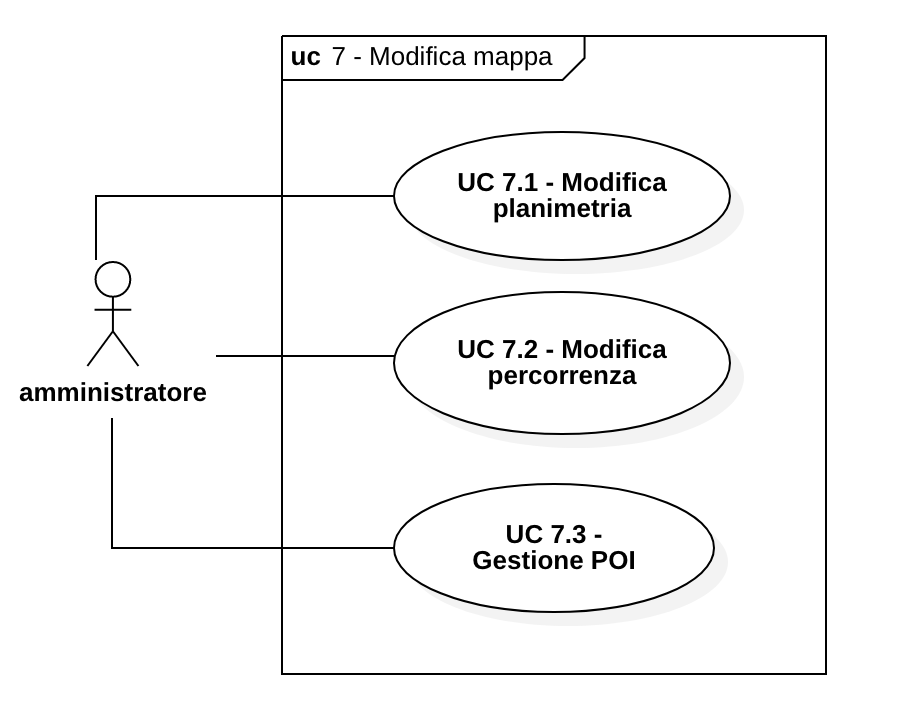
\includegraphics[scale=0.52]{res/images/uc7.png}
	\caption{UC7 - Gestione mappa}
\end{figure}

\begin{itemize}
	\item 	\textbf{Attori primari:} amministratore;
	\item 	\textbf{Precondizioni:} l'amministratore è autenticato nel sistema e viene reso disponibile dal sistema un pulsante per la modifica della mappa;
	\item 	\textbf{Postcondizioni:} la mappa è stata modificata dall'amministratore;
	\item 	\textbf{Scenario principale:} l'amministratore una volta autenticato preme il pulsante per la gestione della mappa dal quale può effettuare le seguenti operazioni:
	\begin{itemize}
		\item modificare la mappa (UC7.1);
		\item gestire i punti d'interesse (UC7.4);
	\end{itemize}
	\item 	\textbf{Descrizione:} l'amministratore ha il compito di gestire la mappa e tenere aggiornati i cambiamenti reali del magazzino nell'applicativo.
\end{itemize}


\subsubsection{UC7.1 - Modifica mappa}
\begin{itemize}
	\item 	\textbf{Attori primari:} amministratore;
	\item 	\textbf{Precondizioni:} viene resa disponibile dal sistema l'interfaccia per la modifica della mappa;
	\item 	\textbf{Postcondizioni:} la mappa è stata modificata dall'amministratore;
	\item 	\textbf{Scenario principale:} l'amministratore dopo aver premuto il pulsante per la modifica, visualizza l'interfaccia per gestire i cambiamenti della mappa tra cui può scegliere tramite un menù a tendina se:
	\begin{itemize}
		\item modificare la \gls{planimetria}\textsubscript{G} del magazzino (UC7.2);
		\item modificare la \gls{percorrenza}\textsubscript{G} del magazzino, per esempio i sensi di marcia (UC7.3);
		\item gestire i \acrshort{POI}\textsubscript{A} (UC7.4);
	\end{itemize}
	e viene visualizzata l'intera mappa (UC6).
Terminata la modifica, l'amministratore salva tramite l'apposito pulsante di conferma;
	\item 	\textbf{Descrizione:} l'amministratore ha il compito di tenere aggiornata la mappa dai cambiamenti reali del magazzino, modificandone la \gls{planimetria}\textsubscript{G}, la \gls{percorrenza}\textsubscript{G} e i \acrshort{POI}\textsubscript{A} presenti.
	\item 	\textbf{Specializzazione:} 
	\begin{itemize}
		\item UC7.2 - Modifica \gls{planimetria}\textsubscript{G}
		\item UC7.3 - Modifica \gls{percorrenza}\textsubscript{G}
		\item UC7.4 - Gestione \acrshort{POI}\textsubscript{A}
	\end{itemize}
	\item \textbf{Estensione}:
	\begin{itemize}
		\item UC7.5 - Visualizzazione messaggio d'errore operazione non permessa.
	\end{itemize}
\end{itemize}


\subsubsection{UC7.2 - Modifica planimetria}
\begin{itemize}
	\item 	\textbf{Attori primari:} amministratore;
	\item 	\textbf{Precondizioni:} viene resa disponibile dal sistema l'interfaccia per la modifica della \gls{planimetria}\textsubscript{G} della mappa;
	\item 	\textbf{Postcondizioni:} la mappa è stata modificata dall'amministratore;
	\item 	\textbf{Scenario principale:} vengono visualizzati degli strumenti per la modifica della \gls{planimetria}\textsubscript{G}:
	\begin{itemize}
		\item ampliamento;
		\item riduzione;
		\item aggiunta, rimozione e modifica zone non transitabili.
	\end{itemize}
	Una volta raggiunto il risultato desiderato, l'amministratore conferma tramite il pulsante di salvataggio;
	\item 	\textbf{Descrizione:} il magazzino, con il passare del tempo, può subire dei cambiamenti nella \gls{planimetria}\textsubscript{G}. Possono venire modificati:
	\begin{itemize}
		\item la dimensione del magazzino (ampliarlo o diminuirlo);
		\item le zone in cui non è permessa la transizione dei mezzi (scaffali, muri, elementi e zone del magazzino che non prevedono il transito di un muletto).
	\end{itemize}
\end{itemize}

\subsubsection{UC7.3 - Modifica percorrenza}
\begin{itemize}
	\item 	\textbf{Attori primari:} amministratore;
	\item 	\textbf{Precondizioni:}  l'amministratore è autenticato nel sistema e viene reso disponibile dal sistema l'interfaccia per la modifica della \gls{percorrenza}\textsubscript{G} della mappa;
	\item 	\textbf{Postcondizioni:} la mappa è stata modificata dall'amministratore;
	\item 	\textbf{Scenario principale:} viene visualizzata la mappa con le caratteristiche che ogni area di \gls{percorrenza}\textsubscript{G} ha (senso di marcia e numero massimo di unità). L'amministratore deve premere sopra la zona che intende cambiare per aprire un pop-up e inserire gli aggiornamenti. Una volta raggiunto il risultato desiderato, l'amministratore conferma tramite il pulsante di salvataggio;
	\item 	\textbf{Descrizione:} il magazzino può subire dei cambiamenti nella \gls{percorrenza}\textsubscript{G}. Sarà possibile modificare per ogni area:
	\begin{itemize}
		\item il senso di marcia;
		\item il numero massimo di unità transitabili contemporaneamente.
	\end{itemize}
\end{itemize}

\subsubsection{UC7.4 - Gestione POI}

\begin{figure}[H]
	\centering
	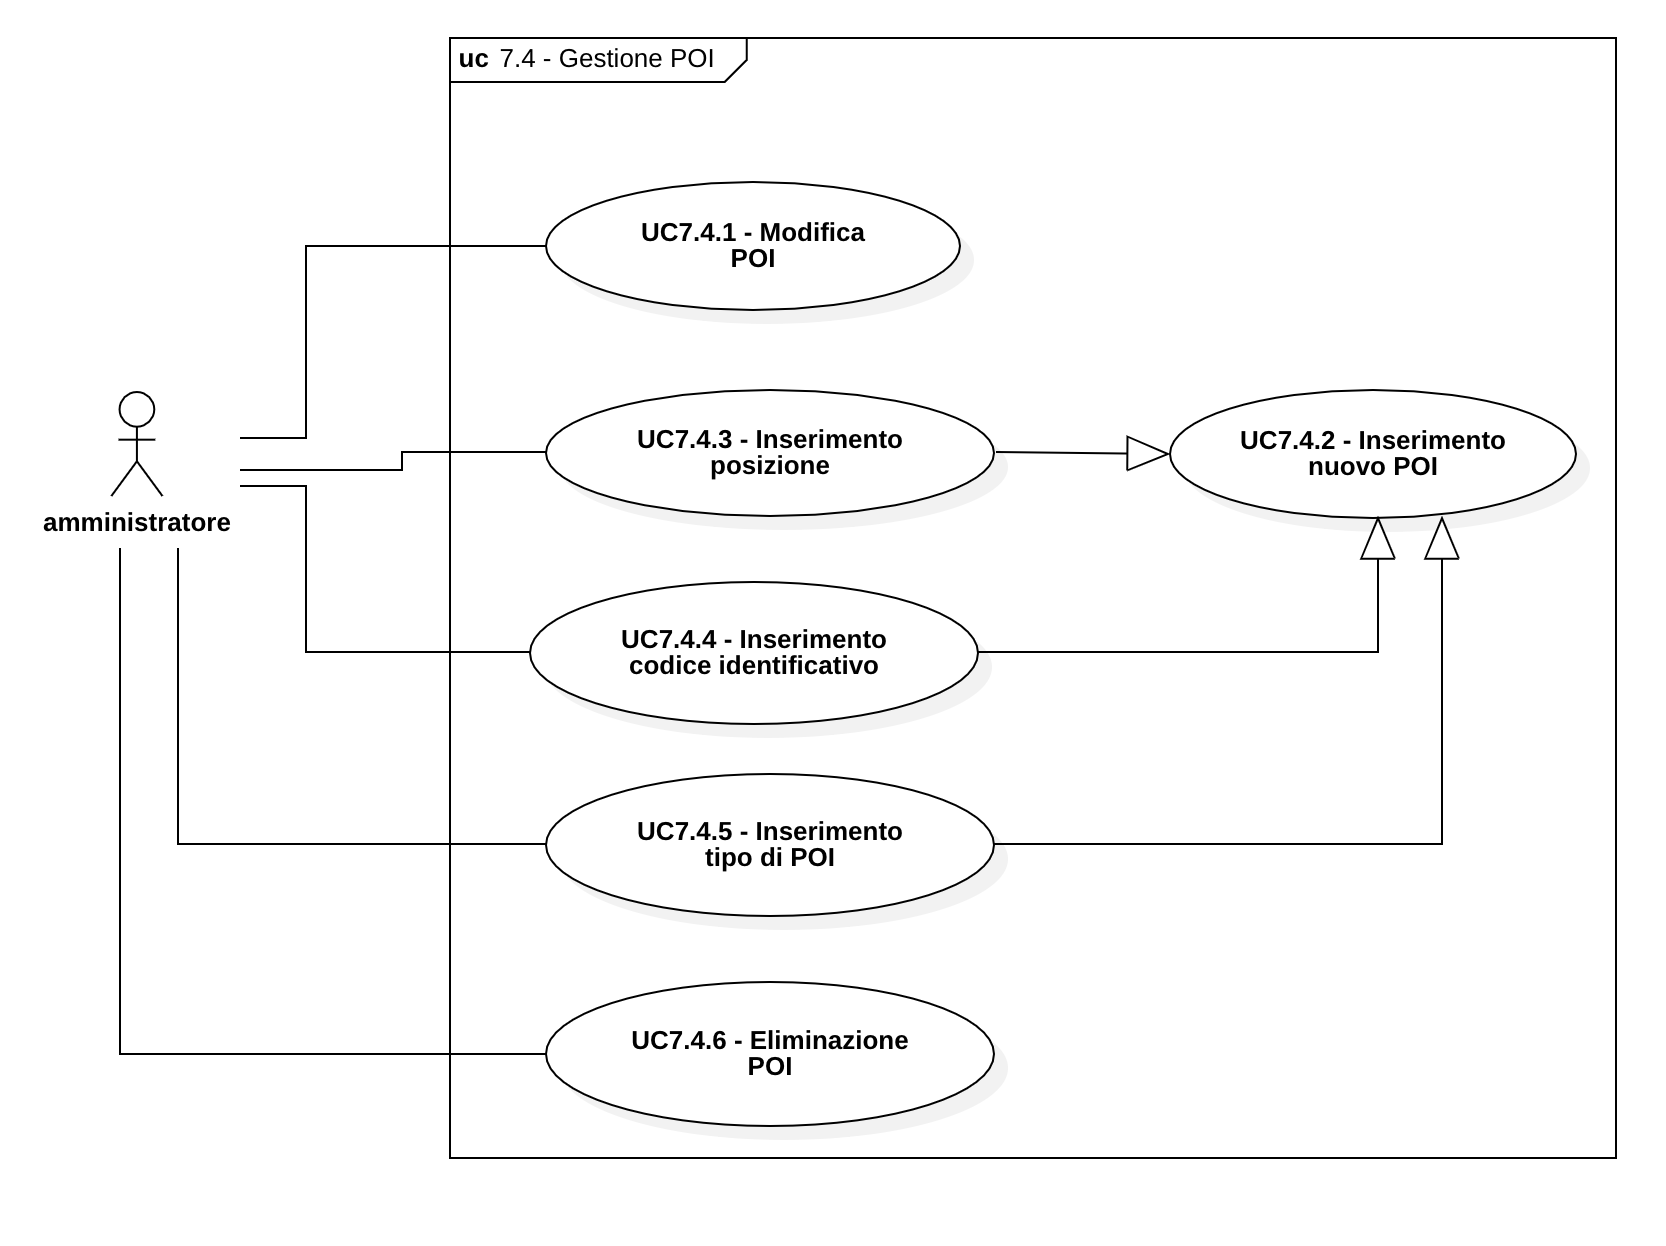
\includegraphics[scale=0.52]{res/images/uc7-4.png}
	\caption{UC7.4 - Gestione POI}
\end{figure}

\begin{itemize}
	\item 	\textbf{Attori primari:} amministratore;
	\item 	\textbf{Precondizioni:} l'amministratore è autenticato nel sistema e viene reso disponibile dal sistema l'interfaccia per la modifica dei \acrshort{POI}\textsubscript{A};
	\item 	\textbf{Postcondizioni:} nella mappa sono comparsi i cambiamenti dei \acrshort{POI}\textsubscript{A}; 
	\item 	\textbf{Scenario principale:} l'amministratore dopo aver premuto il pulsante per la modifica dei POI, visualizza le opzioni tra cui può scegliere le operazioni da eseguire:
	\begin{itemize}
		\item modificare la posizione di un \acrshort{POI}\textsubscript{A} esistente (UC7.4.1);
		\item aggiungere un nuovo \acrshort{POI}\textsubscript{A} nella mappa (UC7.4.2);
		\item eliminare un \acrshort{POI}\textsubscript{A} esistente (UC7.4.6).
	\end{itemize}
	\item 	\textbf{Descrizione:} è possibile che sia necessaria la modifica dei punti di interesse nella mappa, l'amministratore ha appunto il compito di aggiungerne, modificarne o eliminarli in base alle esigenze del magazzino. Il responsabile deve tenere presente i vincoli del magazzino altrimenti non sarà permessa l'operazione:
	\begin{itemize}
		\item almeno una base;
		\item almeno un \acrshort{POI}\textsubscript{A} di carico.
	\end{itemize}
\end{itemize}

\paragraph{UC7.4.1 - Modifica posizione di un \acrshort{POI}\textsubscript{A} esistente}

\begin{itemize}
	\item 	\textbf{Attori primari:} amministratore;
	\item 	\textbf{Precondizioni:} l'amministratore ha selezionato l'opzione tra il menu della modifica dei \acrshort{POI}\textsubscript{A} per il cambiamento della posizione di un \acrshort{POI}\textsubscript{A} esistente;
	\item 	\textbf{Postcondizioni:} il \acrshort{POI}\textsubscript{A} selezionato ha cambiato posizione nella mappa; 
	\item 	\textbf{Scenario principale:} l'amministratore dopo aver premuto il pulsante per la modifica della posizione di un \acrshort{POI}\textsubscript{A} esistente, visualizza la mappa (UC6) con tutti i \acrshort{POI}\textsubscript{A} nella loro posizione, seleziona quello che gli interessa e lo sposta nella posizione aggiornata;
	\item 	\textbf{Descrizione:} l'amministratore può dover cambiare la posizione di alcuni \acrshort{POI}\textsubscript{A} già esistenti all'interno del magazzino.
\end{itemize}
\paragraph{UC7.4.2 - Inserimento nuovo POI}

\begin{itemize}
	\item 	\textbf{Attori primari:} amministratore;
	\item 	\textbf{Precondizioni:} l'amministratore ha selezionato l'opzione, tra il menu, dell'aggiunta di un nuovo \acrshort{POI}\textsubscript{A};
	\item 	\textbf{Postcondizioni:} viene creato il nuovo \acrshort{POI}\textsubscript{A} nella mappa;
	\item 	\textbf{Scenario principale:} l'amministratore dopo aver premuto il pulsante per l'aggiunta di un nuovo POI, visualizzerà l'interfaccia per la creazione del nuovo punto d'interesse;
	\item 	\textbf{Descrizione:} per inserire un nuovo \acrshort{POI}\textsubscript{A} all'interno della mappa devono essere specificati:
	\begin{itemize}
		\item codice identificativo;
		\item posizione nella mappa;
		\item tipo di \acrshort{POI}\textsubscript{A} (carico, scarico, base);
	\end{itemize}
	\item 	\textbf{Specializzazione:}
	\begin{itemize}
		\item UC7.4.3 - Inserimento posizione;
		\item UC7.4.4 - Inserimento codice identificativo;
		\item UC7.4.5 - Inserimento tipo di \acrshort{POI}\textsubscript{A}.
	\end{itemize}
\end{itemize}

\paragraph{UC7.4.3 - Inserimento posizione}
\begin{itemize}
	\item 	\textbf{Attori primari:} amministratore;
	\item 	\textbf{Precondizioni:} l'amministratore visualizza la mappa per l'inserimento dei dati del nuovo \acrshort{POI}\textsubscript{A}.
	\item 	\textbf{Postcondizioni:} l'amministratore ha inserito il \acrshort{POI}\textsubscript{A} all'interno della mappa; 
	\item 	\textbf{Scenario principale:}
	\begin{itemize}
		\item visualizza la mappa (UC6);
		\item preme nel punto in cui vuole inserire il \acrshort{POI}\textsubscript{A};
		\item conferma l'inserimento premendo un pulsante apposito;
	\end{itemize}
	\item 	\textbf{Descrizione:} per completare l'aggiunta, l'amministratore deve posizionare il \acrshort{POI}\textsubscript{A} nella mappa.

\end{itemize}

\paragraph{UC7.4.4 - Inserimento codice identificativo}
\begin{itemize}
	\item 	\textbf{Attori primari:} amministratore;
	\item 	\textbf{Precondizioni:} l'amministratore visualizza il \gls{form}\textsubscript{G} per l'inserimento del codice identificativo del nuovo \acrshort{POI}\textsubscript{A};
	\item 	\textbf{Postcondizioni:} l'amministratore ha inserito il codice identificativo del nuovo \acrshort{POI}\textsubscript{A}; 
	\item 	\textbf{Scenario principale:} l'amministratore inserisce il codice identificativo del nuovo \acrshort{POI}\textsubscript{A} nell'apposito \gls{form}\textsubscript{G};
	\item 	\textbf{Descrizione:} per completare l'aggiunta, l'amministratore deve assegnare un codice identificativo al nuovo \acrshort{POI}\textsubscript{A}.

\end{itemize}

\paragraph{UC7.4.5 - Inserimento tipo POI}
\begin{itemize}
	\item 	\textbf{Attori primari:} amministratore;
	\item 	\textbf{Precondizioni:} l'amministratore visualizza il \gls{form}\textsubscript{G} per l'inserimento del tipo di \acrshort{POI}\textsubscript{A};
	\item 	\textbf{Postcondizioni:} viene creato il nuovo \acrshort{POI}\textsubscript{A} nella mappa; 
	\item 	\textbf{Scenario principale:} l'amministratore inserisce il tipo di \acrshort{POI}\textsubscript{A} e conferma;
	\item 	\textbf{Descrizione:} per completare l'aggiunta, l'amministratore deve assegnare il tipo di \acrshort{POI}\textsubscript{A} nella mappa:
	\begin{itemize}
		\item scarico;
		\item carico;
		\item base.
	\end{itemize}

\end{itemize}

\paragraph{UC7.4.6 - Eliminazione POI}
\begin{itemize}
	\item 	\textbf{Attori primari:} amministratore;
	\item 	\textbf{Precondizioni:} l'amministratore ha selezionato l'opzione tra il menu per l'eliminazione di un \acrshort{POI}\textsubscript{A} esistente e visualizza la mappa con tutti i \acrshort{POI}\textsubscript{A};
	\item 	\textbf{Postcondizioni:} viene eliminato un \acrshort{POI}\textsubscript{A} dalla mappa e dalla lista; 
	\item 	\textbf{Scenario principale:} seleziona dalla mappa il \acrshort{POI}\textsubscript{A} di interesse e conferma, attraverso un apposito pulsante, l'eliminazione;
	\item 	\textbf{Descrizione:} si vuole eliminare un \acrshort{POI}\textsubscript{A} esistente dalla mappa.
\end{itemize}
\subsubsection{UC7.5 - Visualizzazione messaggio d'errore operazione non permessa}
\begin{itemize}
	\item 	\textbf{Attori primari:} amministratore;
	\item 	\textbf{Precondizioni:} l'amministratore ha tentato una modifica alla mappa esistente;
	\item 	\textbf{Postcondizioni:} è stato visualizzato un messaggio d'errore che informa l'amministratore di aver cercato di fare un'operazione non concessa dal sistema;
	\item 	\textbf{Scenario principale:} l'amministratore tenta di apportare una modifica non concessa alla mappa;
	\item 	\textbf{Descrizione:} alcune operazioni di modifica della mappa non sono concesse, quindi il sistema informa l'amministratore.
\end{itemize}

\subsection{UC8 - Visualizzazione task}

\begin{figure}[H]
	\centering
	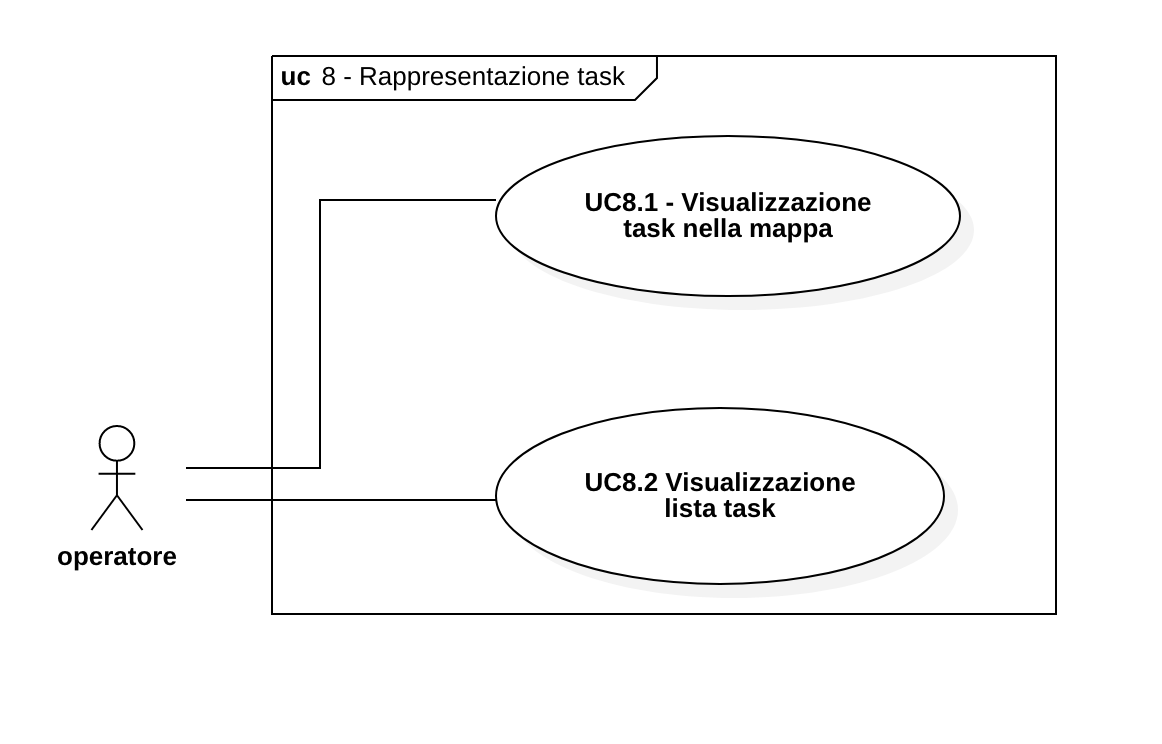
\includegraphics[scale=0.52]{res/images/uc8.png}
	\caption{UC8 - Visualizzazione task}
\end{figure}


\begin{itemize}
	\item 	\textbf{Attori primari:} operatore;
	\item 	\textbf{Precondizioni:} l'operatore è sul muletto che si appresta a svolgere i propri compiti;
	\item 	\textbf{Postcondizioni:} l'operatore ha una visione completa dei suoi compiti;
	\item 	\textbf{Scenario principale:} il sistema rende disponibile la visualizzazione di tutte le \gls{task}\textsubscript{G} assegnate all'operatore;
	\item 	\textbf{Descrizione:} per compiere il suo lavoro, l'operatore ha bisogno di visualizzare le \gls{task}\textsubscript{G} che gli sono assegnate e la loro posizione, così da poter scaricare la merce nel luogo corretto.

\end{itemize}

\subsubsection{UC8.1 - Visualizzazione \gls{task}\textsubscript{G} nella mappa}
\begin{itemize}
	\item 	\textbf{Attori primari:} operatore;
	\item 	\textbf{Precondizioni:} l'operatore è sul muletto che si appresta a svolgere i propri compiti;
	\item 	\textbf{Postcondizioni:} vengono visualizzate nella mappa le \gls{task}\textsubscript{G} nella relativa posizione;
	\item 	\textbf{Scenario principale:} l'operatore visualizza la mappa con le \gls{task}\textsubscript{G} assegnatogli;
	\item 	\textbf{Descrizione:} vengono visualizzate nella mappa le \gls{task}\textsubscript{G} nel loro relativo \acrshort{POI}\textsubscript{A};
	\item 	\textbf{Inclusioni:}
	\begin{itemize}
		\item UC8.2 - Evidenziazione prossima \gls{task}\textsubscript{G}.
	\end{itemize}
\end{itemize}

\subsubsection{UC8.2 - Evidenziazione prossima task}
\begin{itemize}
	\item 	\textbf{Attori primari:} operatore;
	\item 	\textbf{Precondizioni:} l'operatore visualizza la mappa con le \gls{task}\textsubscript{G} (UC8.1);
	\item 	\textbf{Postcondizioni:} viene evidenziata nella mappa la prossima \gls{task}\textsubscript{G} da svolgere;
	\item 	\textbf{Scenario principale:} viene visualizzata nella mappa la prossima \gls{task}\textsubscript{G} con un colore diverso, nella posizione in cui l'operatore deve recarsi;
	\item 	\textbf{Descrizione:} per facilitare il compito dell'operatore, il  \acrshort{POI}\textsubscript{A} relativo alla prossima \gls{task}\textsubscript{G} da soddisfare viene evidenziato con un colore diverso dalle altre \gls{task}\textsubscript{G} all'interno della mappa.

\end{itemize}

\subsubsection{UC8.3 - Visualizzazione lista di task}
\begin{itemize}
	\item 	\textbf{Attori primari:} operatore;
	\item 	\textbf{Precondizioni:} l'operatore è sul muletto che svolge il suo lavoro e sta visualizzando la mappa con le \gls{task}\textsubscript{G} (UC8.1);
	\item 	\textbf{Postcondizioni:} viene visualizzata una lista di tutte le \gls{task}\textsubscript{G} da eseguire;
	\item 	\textbf{Scenario principale:} sotto alla mappa del magazzino, viene visualizzata una lista di tutte le \gls{task}\textsubscript{G} che l'operatore deve soddisfare;
	\item 	\textbf{Descrizione:} per facilitare il compito dell'operatore, viene visualizzata una lista di tutte le \gls{task}\textsubscript{G} che deve soddisfare con il relativo codice identificativo.
\end{itemize}

\subsection{UC9 - Segnalazione del completamento di una task}
\begin{itemize}
	\item 	\textbf{Attori primari:} operatore;
	\item 	\textbf{Precondizioni:} l'operatore ha raggiunto e soddisfatto una \gls{task}\textsubscript{G};
	\item 	\textbf{Postcondizioni:} il sistema ha registrato il completamento della \gls{task}\textsubscript{G} che verrà cancellata dalla lista completa di tutte le \gls{task}\textsubscript{G} da soddisfare e da quella personale dell'operatore;
	\item 	\textbf{Scenario principale:} l'operatore clicca sul \acrshort{POI}\textsubscript{A} evidenziato in UC8.3 e conferma l'avvenuto scarico;
	\item 	\textbf{Descrizione:} l'operatore ha scaricato la merce nel punto destinato, quindi deve segnalare di aver completato la \gls{task}\textsubscript{G} per poter proseguire con la prossima.

\end{itemize}

\subsection{UC10 - Visualizzazione spostamenti del pilota automatico}
\begin{itemize}
	\item 	\textbf{Attori primari:} operatore;
	\item 	\textbf{Precondizioni:} l'operatore è a bordo di un muletto in cui è attiva la guida automatica;
	\item 	\textbf{Postcondizioni:} l'operatore visualizza la direzione degli spostamenti del pilota automatico mentre è a bordo del muletto;
	\item 	\textbf{Scenario principale:} il sistema accende le icone delle quattro frecce direzionali e dello start/stop in base agli spostamenti che intende effettuare;
	\item 	\textbf{Descrizione:} le unità possono essere guidate dal pilota automatico, ma l'operatore deve controllare gli spostamenti che il sistema ha intenzione di effettuare.

\end{itemize}
 
\subsection{UC11 - Gestione guida}

\begin{figure}[H]
	\centering
	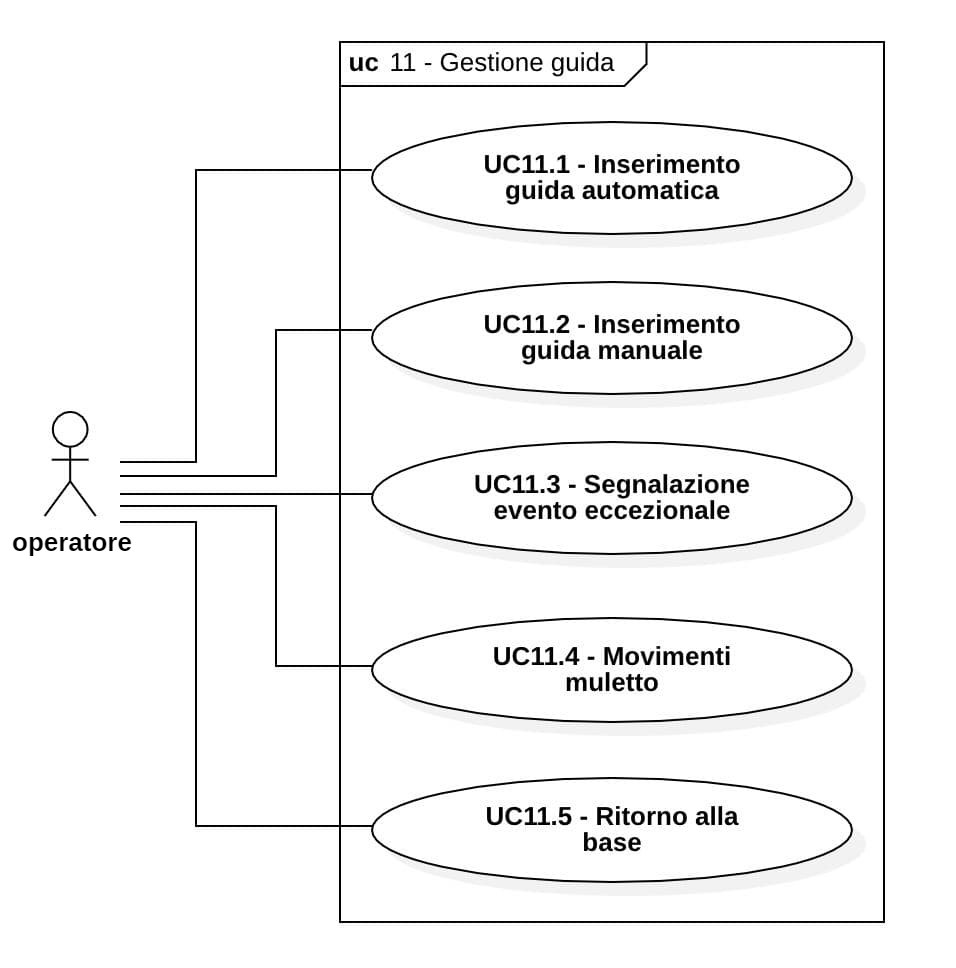
\includegraphics[scale=0.52]{res/images/uc11.png}
	\caption{ UC11 - Gestione guida}
\end{figure}

\begin{itemize}
	\item 	\textbf{Attori primari:} operatore;
	\item 	\textbf{Precondizioni:} l'operatore si è autenticato nel sistema ed è pronto a svolgere il suo compito;
	\item 	\textbf{Postcondizioni:} l'operatore ha interagito correttamente con il sistema; 
	\item 	\textbf{Scenario principale:} l'operatore effettua le operazioni per la gestione della guida del muletto, ossia:
	\begin{itemize}
		\item l'inserimento della guida autonoma se è in modalità di guida manuale (UC11.1);
		\item l'inserimento della guida manuale se è in modalità di guida autonoma (UC11.2);
		\item la segnalazione di un evento eccezionale, per esempio ingorghi, collisioni o malfunzionamenti (UC11.3);
		\item lo spostamento del muletto all'interno della mappa (UC11.4);
	\end{itemize}
	\item 	\textbf{Descrizione:} l'operatore si appresta a guidare o supervisionare la guida del muletto. 

\end{itemize}

\subsubsection{UC11.1 - Inserimento guida automatica}
\begin{itemize}
	\item 	\textbf{Attori primari:} operatore;
	\item 	\textbf{Precondizioni:} l'operatore sta guidando manualmente il muletto;
	\item 	\textbf{Postcondizioni:} il sistema controlla il movimento del muletto;
	\item 	\textbf{Scenario principale:} l'operatore preme il pulsante apposito per il passaggio a guida automatica;
	\item 	\textbf{Descrizione:} i muletti possono essere guidati sia in modo automatico dal sistema che manuale, in base alle esigenze dell'operatore.
\end{itemize}

\subsubsection{UC11.2 - Inserimento guida manuale}
\begin{itemize}
	\item 	\textbf{Attori primari:} operatore;
	\item 	\textbf{Precondizioni:} il sistema centrale controlla il movimento del muletto;
	\item 	\textbf{Postcondizioni:} l'operatore guida il muletto manualmente; 
	\item 	\textbf{Scenario principale:} l'operatore preme il pulsante apposito per il passaggio a guida manuale;
	\item 	\textbf{Descrizione:} i muletti possono essere guidati sia in modo automatico dal sistema che manuale, in base alle esigenze dell'operatore.
\end{itemize}

\subsubsection{UC11.3 - Segnalazione evento eccezionale}
\begin{itemize}
	\item 	\textbf{Attori primari:} operatore;
	\item 	\textbf{Precondizioni:} il muletto si sta muovendo all'interno della mappa;
	\item 	\textbf{Postcondizioni:} un evento eccezionale è stato segnalato al sistema centrale; 
	\item 	\textbf{Scenario principale:} l'operatore preme il pulsante apposito per la segnalazione di un evento eccezionale;
	\item 	\textbf{Descrizione:} durante la guida possono verificarsi degli eventi eccezionali per esempio collisioni, ingorghi o malfunzionamenti del muletto. L'operatore deve segnalarli e il sistema centrale ha il compito di propagarli al responsabile e amministratore affinché possano essere gestiti.

\end{itemize}

\subsubsection{UC11.4 - Spostamento muletto}

\begin{figure}[H]
	\centering
	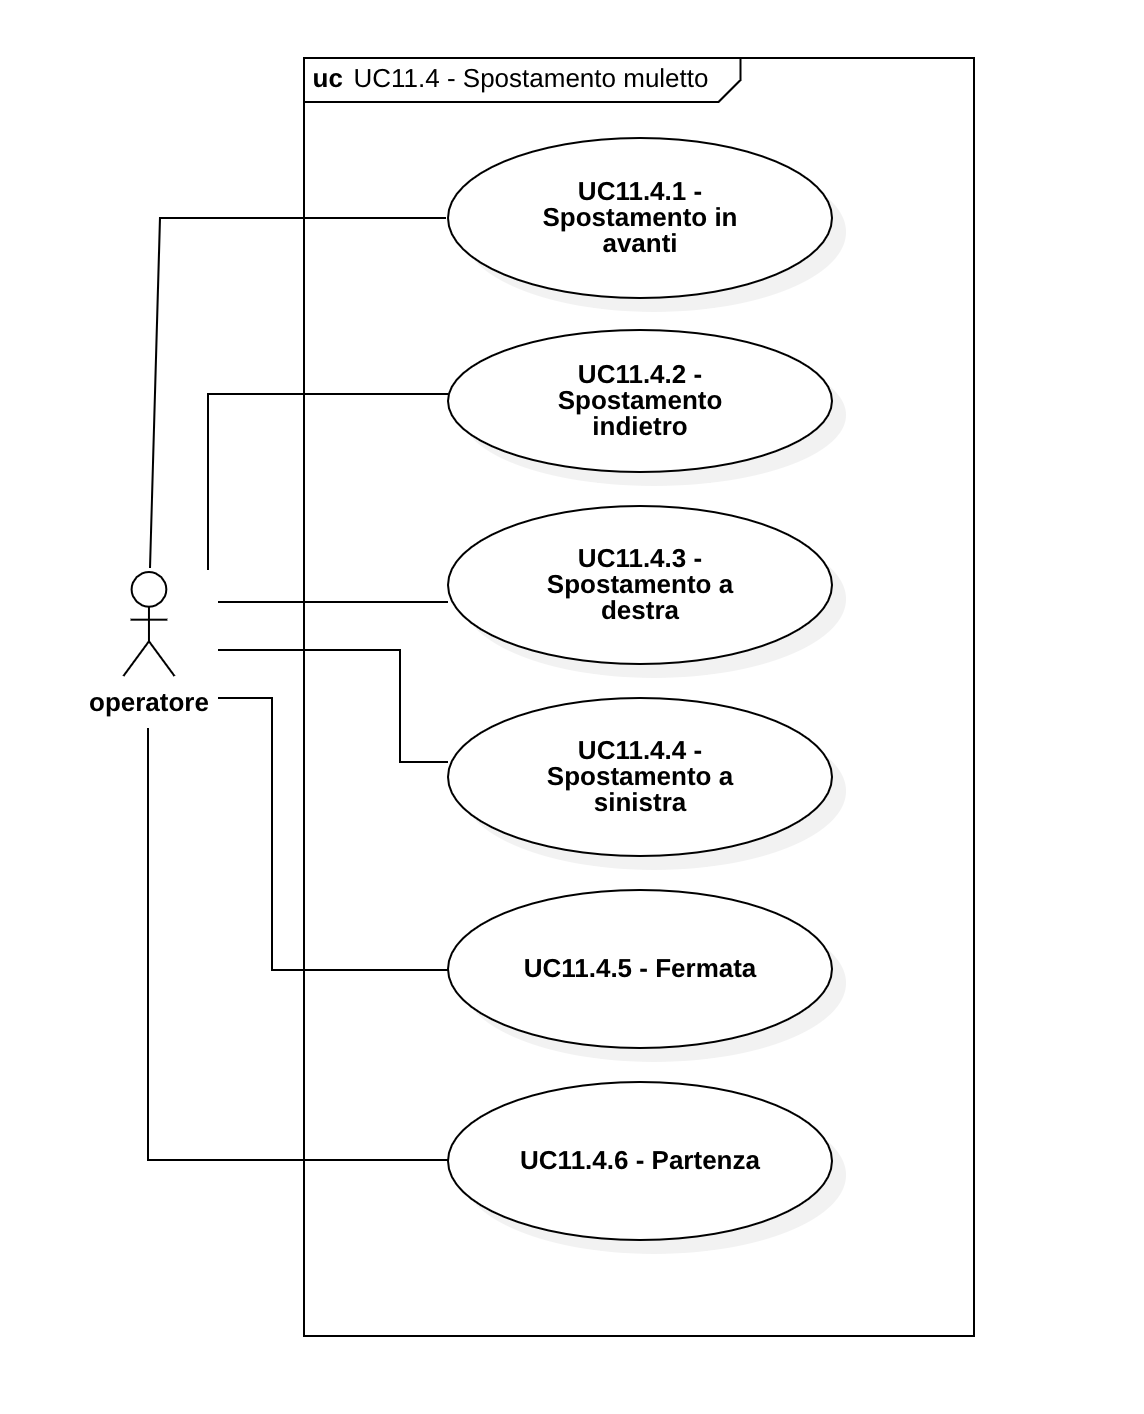
\includegraphics[scale=0.52]{res/images/uc11-4.png}
	\caption{UC11.4 - Spostamento muletto}
\end{figure}

\begin{itemize}
	\item 	\textbf{Attori primari:} operatore;
	\item 	\textbf{Precondizioni:} l'operatore controlla lo spostamento del muletto, la modalità di guida è quella manuale;
	\item 	\textbf{Postcondizioni:} il muletto ha effettuato uno spostamento;
	\item 	\textbf{Scenario principale:}il sistema rende disponibile l'interfaccia per lo spostamento del muletto, ossia le quattro frecce direzionali e un pulsante di start/stop. L'operatore può eseguire le seguenti operazioni:
	\begin{itemize}
		\item spostamento in avanti (UC1.4.1); 
		\item spostamento indietro (UC1.4.2);
		\item spostamento a destra (UC1.4.3);
		\item spostamento a sinistra (UC1.4.4);
		\item la fermata del muletto (UC1.4.5);
		\item la partenza del muletto (UC1.4.6);
	\end{itemize}
	\item 	\textbf{Descrizione:} i muletti possono intraprendere degli spostamenti all'interno della mappa per raggiungere i vari \acrshort{POI}\textsubscript{A}. Essi possono essere controllati manualmente dall'operatore.
\end{itemize}


\paragraph{UC11.4.1 - Spostamento in avanti}
\begin{itemize}
	\item 	\textbf{Attori primari:} operatore;
	\item 	\textbf{Precondizioni:} l'operatore controlla il movimento del muletto;
	\item 	\textbf{Postcondizioni:} il muletto ha effettuato uno spostamento in avanti; 
	\item 	\textbf{Scenario principale:} l'operatore preme la freccia in alto;
	\item 	\textbf{Descrizione:} l'operatore intende far effettuare al muletto uno spostamento in avanti, ripetto alla propria direzione, all'interno della mappa.

\end{itemize}

\paragraph{UC11.4.2 - Spostamento indietro}
\begin{itemize}
	\item 	\textbf{Attori primari:} operatore;
	\item 	\textbf{Precondizioni:} l'operatore controlla il movimento del muletto;
	\item 	\textbf{Postcondizioni:} il muletto ha effettuato uno spostamento indietro; 
	\item 	\textbf{Scenario principale:} l'operatore preme la freccia in basso;
	\item 	\textbf{Descrizione:} l'operatore intende far effettuare al muletto uno spostamento indietro, ripetto alla propria direzione, all'interno della mappa.
\end{itemize}

\paragraph{UC11.4.3 - Spostamento a destra}
\begin{itemize}
	\item 	\textbf{Attori primari:} operatore;
	\item 	\textbf{Precondizioni:} l'operatore controlla il movimento del muletto;
	\item 	\textbf{Postcondizioni:} il muletto ha effettuato uno spostamento a destra; 
	\item 	\textbf{Scenario principale:} l'operatore preme la freccia a destra;
	\item 	\textbf{Descrizione:} l'operatore intende far effettuare al muletto uno spostamento a destra, ripetto alla propria direzione, all'interno della mappa.

\end{itemize}

\paragraph{UC11.4.4 - Spostamento a sinistra}
\begin{itemize}
	\item 	\textbf{Attori primari:} operatore;
	\item 	\textbf{Precondizioni:} l'operatore controlla il movimento del muletto;
	\item 	\textbf{Postcondizioni:} il muletto ha effettuato uno spostamento a sinistra; 
	\item 	\textbf{Scenario principale:} l'operatore preme la freccia a sinistra;
	\item 	\textbf{Descrizione:} l'operatore intende far effettuare al muletto uno spostamento a sinistra, ripetto alla propria direzione, all'interno della mappa.
\end{itemize}


\paragraph{UC11.4.5 - Fermata}
\begin{itemize}
	\item 	\textbf{Attori primari:} operatore;
	\item 	\textbf{Precondizioni:} l'operatore controlla il movimento del muletto, esso è in azione e si sta muovendo; Il sistema rende disponibile il pulsante di stop;
	\item 	\textbf{Postcondizioni:} il muletto è fermo all'interno della mappa o in base;
	\item 	\textbf{Scenario principale:} l'operatore preme il pulsante di stop;
	\item 	\textbf{Descrizione:} quando il muletto è in movimento è possibile fermarne il moto. Per ripartire sarà necessario azionare il pulsante di partenza (UC11.4.6).
\end{itemize}


\paragraph{UC11.4.6 - Partenza}
\begin{itemize}
	\item 	\textbf{Attori primari:} operatore;
	\item 	\textbf{Precondizioni:} l'operatore controlla il movimento del muletto, esso è stato precedentemente fermato (UC11.4.5) oppure si trova alla base pronto per iniziare a lavorare; il sistema rende disponibile il pulsante di start;
	\item 	\textbf{Postcondizioni:} il muletto è in azione;
	\item 	\textbf{Scenario principale:} l'operatore preme il pulsante di start;
	\item 	\textbf{Descrizione:} il muletto può essere azionato perchè l'operatore intende partire:
	\begin{itemize}
		\item dalla base per raggiungere i \acrshort{POI}\textsubscript{A} da soddisfare;
		\item dopo aver effettuato una fermata a causa di un imprevisto o dello scarico delle merci (UC11.4.5).
	\end{itemize}
\end{itemize}


\subsubsection{UC11.5 - Ritorno alla base}
\begin{itemize}
	\item 	\textbf{Attori primari:} operatore;
	\item 	\textbf{Precondizioni:} l'operatore ha finito il turno e ha eseguito tutte le \gls{task}\textsubscript{G} assegnatoli. Il sistema rende disponibile un pulsante per il ritorno alla base;
	\item 	\textbf{Postcondizioni:} il muletto è nel punto della mappa base;
	\item 	\textbf{Scenario principale:} l'operatore preme nell'apposito pulsante per il ritorno alla base. Se la guida è impostata in manuale dovrà guidare fino al punto, altrimenti il sistema lo porta a destinazione;
	\item 	\textbf{Descrizione:} quando ha finito il turno, l'operatore deve ritornare alla base dove lascia il proprio mezzo per essere usato da un altro operatore.
\end{itemize}

\subsection{UC12 - Visualizzazione lista completa di POI}
\begin{itemize}
	\item 	\textbf{Attori primari:} amministratore, responsabile;
	\item 	\textbf{Precondizioni:} gli utenti sono autenticati;
	\item 	\textbf{Postcondizioni:} viene visualizzata la lista completa dei \acrshort{POI}\textsubscript{A} presenti nella mappa;
	\item 	\textbf{Scenario principale:} vicino alla visualizzazione della mappa (UC6), vi è un pulsante apposito per visualizzare la lista completa di \acrshort{POI}\textsubscript{A} presenti nel magazzino;
	\item 	\textbf{Descrizione:} per tener traccia di tutti i \acrshort{POI}\textsubscript{A} con il proprio tipo (carico, scarico, base) presenti nella mappa, il sistema rende disponibile la lista.

\end{itemize}

\subsection{UC13 - Visualizzazione lista completa di task}
\begin{itemize}
	\item 	\textbf{Attori primari:} responsabile;
	\item 	\textbf{Precondizioni:} l'utente è autenticato come utente responsabile;
	\item 	\textbf{Postcondizioni:} il responsabile visualizza la lista di \gls{task}\textsubscript{G};
	\item 	\textbf{Scenario principale:} il responsabile clicca sul bottone apposito per poter visualizzare la lista completa delle \gls{task}\textsubscript{G};
	\item 	\textbf{Descrizione:} il responsabile necessita di visualizzare tutte le \gls{task}\textsubscript{G} che sono state create per tenere sotto controllo quali compiti vengono soddisfatti.

\end{itemize}

\subsection{UC14 - Gestione unità}

\begin{figure}[H]
	\centering
	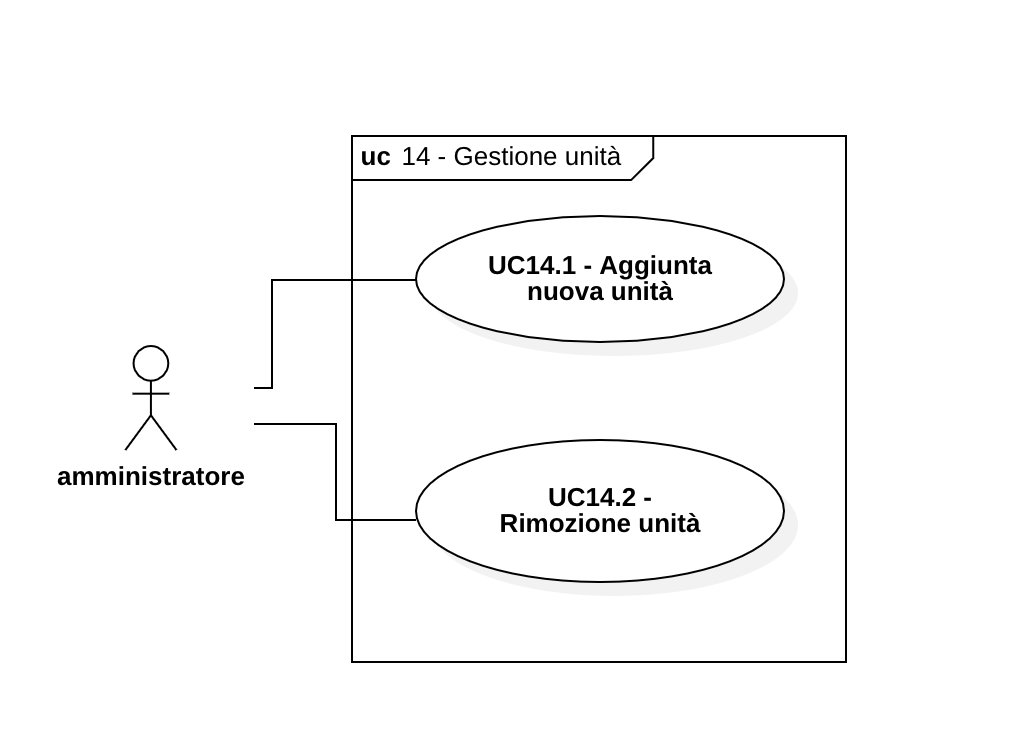
\includegraphics[scale=0.52]{res/images/uc14.png}
	\caption{UC14 - Gestione unità}
\end{figure}

\begin{itemize}
	\item 	\textbf{Attori primari:} amministratore;
	\item 	\textbf{Precondizioni:} l'utente è autenticato come amministratore e viene resa disponibile l'interfaccia per la gestione delle unità;
	\item 	\textbf{Postcondizioni:} è cambiata la quantità di unità gestite dal sistema;
	\item 	\textbf{Scenario principale:} l'amministratore dopo aver premuto il pulsante per la gestione delle unità, visualizza le operazioni che può effettuare:
	\begin{itemize}
		\item l'aggiunta di un nuovo mezzo (UC14.1);
		\item la rimozione di un mezzo esistente (UC14.2);
	\end{itemize}
	\item 	\textbf{Descrizione:} ogni unità (muletto) deve essere identificata all'interno del magazzino attraverso il proprio codice identificativo. L'amministratore ha il compito di gestire l'aggiunta di un nuovo muletto all'interno del magazzino e la sua eliminazione.
\end{itemize}

\subsubsection{UC14.1 - Aggiunta nuova unità}
\begin{itemize}
	\item 	\textbf{Attori primari:} amministratore;
	\item 	\textbf{Precondizioni:} l'amministratore sta visualizzando l'interfaccia per l'aggiunta di un nuovo mezzo;
	\item 	\textbf{Postcondizioni:} è stata aggiunta un'unità all'interno del sistema con il relativo codice identificativo;
	\item 	\textbf{Scenario principale:} l'amministratore visualizza un \gls{form}\textsubscript{G} per l'inserimento del codice identificativo del muletto e conferma l'aggiunta.
	\item 	\textbf{Descrizione:} quando viene utilizzato un nuovo muletto all'interno del magazzino, esso deve venire registrato nel sistema dall'amministratore assegnandogli un proprio codice identificativo.

\end{itemize}


\subsubsection{UC14.2 - Rimozione unità}
\begin{itemize}
	\item 	\textbf{Attori primari:} amministratore;
	\item 	\textbf{Precondizioni:} l'amministratore sta visualizzando l'interfaccia per la rimozione di un mezzo;
	\item 	\textbf{Postcondizioni:} un'unità è stata rimossa dal sistema;
	\item 	\textbf{Scenario principale:} l'amministratore seleziona l'unità che deve essere rimossa dal sistema e conferma la modifica;
	\item 	\textbf{Descrizione:} quando un muletto all'interno del magazzino non viene più utilizzato ed è dismesso, esso deve venire rimosso dal sistema.
	
\end{itemize}
